\documentclass[twoside,spanish,ESP,MSc]{plantillaLabUPV}
%\documentclass[oneside,spanish,ESP,MSc]{plantillaLabUPV}
\usepackage[T1]{fontenc}
\usepackage[utf8]{inputenc}
\setcounter{secnumdepth}{3}
\setcounter{tocdepth}{3}
\usepackage{color}
\usepackage{babel}
\usepackage{csquotes} %%%%%% YHM
\addto\shorthandsspanish{\spanishdeactivate{~<>}}

\spanishdecimal{.}

\usepackage{amsmath}
\usepackage{amssymb}
\usepackage[unicode=true,
 bookmarks=true,
 breaklinks=false,pdfborder={0 0 0},backref=false,colorlinks=true]
 {hyperref}

% 30 de Mayo 2022 - Actualizacion MANM - SE incluye el DOI y otros URLs en el listado
% \usepackage[backend=biber,style=ieee]{biblatex}
%\usepackage[backend=biber,style=apa]{biblatex} % para lo que soliciten formato APA
%\usepackage[backend=biber,style=geschichtsfrkl]{biblatex} % para lo que soliciten formato Documento
\usepackage{comment}

% \addbibresource{bibiliography/referencia-tesis.bib}



\hypersetup{pdftitle={tesis_david},
 pdfauthor={David Josué Esquivel Godoy},
 pdfsubject={Tesis de Maestria},
 pdfkeywords={tesis, maestria, upvictoria, upv},
 linkcolor=darkblue, citecolor=darkblue, urlcolor=darkblue, linktoc=page}
\usepackage{breakurl}

\makeatletter
%%%%%%%%%%%%%%%%%%%%%%%%%%%%%% User specified LaTeX commands.



\raggedbottom

\@ifundefined{definecolor}
 {\usepackage[usenames]{color}}{}
\definecolor{darkblue}{rgb}{0.0, 0.4, 0.8}

%\usepackage{subfigure}
\usepackage{rotating}
\usepackage{multirow}
\usepackage{longtable}

\usepackage{subfig}
%\usepackage{subfigure}
%\usepackage{ucs} %%%% Comentado por YHM 5Sp2023
%\usepackage{graphicx}

\usepackage{latexsym}

\usepackage{appendix}

\usepackage{array}
\usepackage{float}
\usepackage{rotfloat}
\usepackage{amsthm}

% Comentados por YHM 5Sp2023
%\usepackage{algorithm}
%\usepackage{algorithmic}
%\usepackage{algorithmicx}
%\usepackage[noend]{algpseudocode}
%\usepackage[linesnumbered,ruled]{algorithm2e}


\usepackage{url}
\theoremstyle{definition}
\newtheorem{mydef}{Definition}
\usepackage[withpage]{acronym}
\usepackage{pdfpages}
\captionsetup{labelsep = period}
\usepackage{fancyhdr} 

\usepackage{wrapfig}
\usepackage{ulem} % TAchar cosas
\usepackage{color,soul} % Resaltar
%\usepackage{lanscape} % Resaltar
\usepackage{lscape}
\usepackage{longtable}
%\usepackage{multirow}
%\usepackage{array}
%\newcolumntype{P}[1]{>{\centering\arraybackslash}p{#1}}


% \usepackage[printonlyused,withpage]{acronym}

%%%%%%%%%%%%%%%%%%%%%%%%%%%%%% LyX specific LaTeX commands.
\providecommand{\tabularnewline}{\\}
\newcommand{\lyxdot}{.}
\floatstyle{ruled}
\newfloat{algorithm}{tbp}{loa}
\floatname{algorithm}{Algoritmo}
%%%%%%%%%%%%%%%%%%%%%%%%%%%%%% User specified LaTeX commands.
\titleen {IMPLEMENTATION OF A DEEP FLOW TECHNIQUE HYDROPONIC SYSTEM CONTROLLED BY FUZZY LOGIC AND MONITORED USING INTERNET OF THINGS}
%\title {CONTROL DIFUSO Y MONITOREO DE UN SISTEMA HIDROPÓNICO DE TÉCNICA DE FLUJO PROFUNDO}
\title {DISEÑO Y CONSTRUCCIÓN DE UN SISTEMA HIDROPÓNICO DE TÉCNICA DE FLUJO PROFUNDO CONTROLADO POR LÓGICA DIFUSA Y SUPERVISADO MEDIANTE INTERNET DE LAS COSAS}

\author      	{DAVID JOSU\'{E} ESQUIVEL GODOY}
\department	{ Maestría en Ingeniería}
\departmenten	{ }
\degreein       	{Sistemas Inteligentes}
\degreeinen     	{ }
\city           		{Cd. Victoria, Tamaulipas, M\'{e}xico}
\date           	{\today}
\degreeday     	 {19}
\degreeyear     	{2023}
\degreemonth   	 {Septiembre}
\degreemonthen  	{Febrero}
%\acknowledgmenttoproject {
%Esta investigación fue parcialmente financiada mediante el proyecto ...
%}

%%%%%%%%%%%%%%%%%%%%%%%%%%%%%%%%%%%%%%%%%%%%%
\chair       	{DR. MARCO AURELIO NUÑO MAGANDA}
\chair         	{DR. YAHIR HERNÁNDEZ MIER}
%%%%%%%%%%%%%%%%%%%%%%%%%%%%%%%%%%%%%%%%%%%%%

%\dedication     {Pendiente...}

%%%%%%%%%%%%%%%%%%%%%%%%%%%%%%%%%%%%%%%%%%%%%

\abstract{
\vspace{-.5cm}
\setlength{\parindent}{0cm}
La presente investigación aplica los conocimientos de control para automatizar un sistema hidropónico de técnica de flujo profundo de manera eficiente. El estudio se enfoca en la implementación de un controlador difuso para reducir la intervención humana y minimizar errores, apoyándose en el internet de las cosas para monitorear las variables de interés en los sistemas hidropónicos: el pH, la conductividad eléctrica, la temperatura y la humedad del aire de los cultivos. Se explora el diseño y construcción de un sistema hidropónico con actuadores y sensores adecuados para ajustar los parámetros de interés en tiempo real en el desarrollo de los cultivos. También, se diseña e integra un controlador difuso para la toma de decisiones con interfaces de usuario y de monitoreo. Se muestran además los resultados de experimentos realizados con el controlador difuso para compensar perturbaciones en las distintas variables monitoreadas dentro del sistema hidropónico construido. Igualmente, se aborda la viabilidad económica de la implementación de tecnologías automatizadas, considerando tanto los costos iniciales como los ahorros a largo plazo. Como trabajo complementario relacionado, se propuso un prototipo basado en visión por computadora que permitirá monitorear el crecimiento de las plantas en el sistema hidróponico, el cual será de utilidad para quien esté encargado de controlar dicho crecimiento de manera remonta. Los resultados experimentales muestran que el controlador implementado permite compensar las perturbaciones introducidas durante el funcionamiento del sistema, lo que confirma su viabilidad de su aplicación en el control automático de sistemas hidropónicos de técnica de flujo profundo. El sistema de monitoreo propuesto efectivamente almacena y permite observar en tiempo real por medio de las interfaces en PC y teléfono móvil el comportamiento de las variables importantes para el sistema.
% los análisis resaltan cómo el monitoreo y automatización  de los sistemas hidropónicos puede revolucionar la forma en que se produce alimentos al aumentar la eficiencia, mejorar la calidad y contribuir a la sustentabilidad. 
}

\abstracten{
\vspace{-.5cm}
The present research applies control knowledge to automate a deep flow technique hydroponic system. The study focuses on the implementation of a fuzzy controller to reduce human intervention and minimize errors, relying on the Internet of Things to monitor the variables of interest in hydroponic systems: pH, electrical conductivity, temperature and humidity of the air of crops. The design and construction of a hydroponic system with actuators and sensors suitable for adjusting the parameters of interest in the development of crops in real time is explored. A fuzzy controller for decision making with user and monitoring interfaces is designed and integrated. The results of experiments carried out with the fuzzy controller to compensate for disturbances in the different variables monitored within the constructed hydroponic system are also shown. Likewise, the economic viability of the implementation of automated technologies is addressed, considering both the initial costs and the long-term savings. As a related complementary work, a prototype based on computer vision was proposed that will allow monitoring the growth of plants in the hydroponic system, which will be useful for whoever is in charge of controlling such growth in a remote way. The experimental results show that the implemented controller allows to compensate for the disturbances introduced during the operation of the system, which confirms its viability of its application in the automatic control of hydroponic systems of deep flow technique. The proposed monitoring system effectively stores and allows to observe in real time through the interfaces on PC and mobile phone the behavior of the important variables for the system.



%This research addresses the knowledge about the monitoring and automation of a hydroponic system, as an innovative solution to improve efficiency and productivity in agriculture. The study focuses on how a controller is implemented using the methodology of fuzzy logic and IoT, based on advanced automation technologies, in hydroponic systems can optimize the control of key variables such as pH, electrical conductivity, temperature and humidity of the air of the crops. The research examines the importance of automation in indoor farming techniques, highlighting how technology can reduce human intervention and minimize errors. That said, it explores the design, implementation of sensors and actuators to monitor and adjust environmental parameters in real time. In addition, the integration of the control system is analyzed, as well as the decision-making algorithms and user interfaces and also a detailed study of cases occurred within hydroponic systems. It also addresses the economic viability of the implementation of automated technologies, considering both the initial costs and the long-term savings. Ultimately, the analyses highlight how monitoring and automating hydroponic systems can revolutionize the way food is produced by increasing efficiency, improving quality and contributing to sustainability. 
}

%%%%%%%%%%%%%%%%%%%%%%%%%%%%%%%%%%%%%%%%%%%%%
%\publication{
 
%}

%%%%%%%%%%%%%%%%%%%%%%%%%%%%%%%%%%%%%%%%%%%%%
\acknowledgments{
\bigskip{}
%\setlength{\parindent}{0cm}
%\begin{itemize}
%\begin{doublespace}

Primeramente, agradezco a Dios por haberme acompañado en esta gran aventura mi maestría, por ser mi gran fortaleza y brindarme una vida llena de aprendizajes, increíbles experiencias y sobre todo felicidad.

Le doy sobre todo las gracias a mis padres Domingo y Juana por apoyarme incondicionalmente en todo momento, por inculcarme los valores, y haberme dado la oportunidad de tener mi educación a posgrado en el transcurso de mi vida tal vez unos ya no estén físicamente pero aun así fueron y serán mi mayor ejemplo a seguir.

A mis hermanos Eugenio por ayudarme y aconsejarme en todo lo posible y hasta lo imposible, a Sabina por ser mi alegría en todo momento.

A mis grandes amigos y compañeros que estuvieron para mí y brindarme su confianza y creer en mí, y hacer mi etapa posgrado una experiencia que jamás podría repetirse.

Le agradezco de corazón por el apoyo y dedicación de su tiempo a mis profesores por haber compartido conmigo muchas partes de su conocimiento y sobre todo su amistad Dr. Said, Dr. Pech, Dr. Benjamin y Dr. Rocha.

Gracias a mi director de tesis el Dr. Nuño y mi co-director Dr. Yahir por creer en mí, y haberme brindado la oportunidad de desarrollar mi tesis de posgrado en base a sus enseñanzas.

Mamaina Sabina Castillo Rodríguez que, aunque ya no te encuentres con nosotros físicamente a ti te lo agradezco todo tú fuiste mi más grande ejemplo inigualable por creer en mi hasta los últimos momentos.

%\end{doublespace}
%\end{itemize}
}

%%%%%%%%%%%%%%%%%%%%%%%%%%%%%%%%%%%%%%%%%%%%%
%%%%% NOMENCLATURA %%%%%%%%%%%%%%%%%%%%%%%%%%

\nomenclature{


\def\arraystretch{1.5}
\begin{table}[h]
\begin{tabular}{lll}
\textbf{ACHPA}          & \multicolumn{1}{c}{\textit{}} & Automatically Controlled Hydro-Ponic Agriculture                \\
\textbf{ANFIS}          & \multicolumn{1}{c}{\textit{}} & Adaptive Neuro-Fuzzy Inference System                \\
\textbf{BGR}          & \multicolumn{1}{c}{\textit{}} & Blue Green Red                \\
\textbf{CE}          & \multicolumn{1}{c}{\textit{}} & Conductividad Eléctrica                \\
\textbf{DFT}          & \multicolumn{1}{c}{\textit{}} & Deep Flow Technique               \\
\textbf{DRFT}     &                               & Dynamic Root Floating Technique \\
\textbf{HSV}     &                               & Hue Saturation Value \\
\textbf{Hp}     &                               & Horsepower \\
\textbf{IoT}          & \multicolumn{1}{c}{\textit{}} & Internet of Things                              \\
\textbf{MicroSD}      &                               & Micro tarjeta de memoria Secure Digital         \\
\textbf{MQTT}      &                               & Message Queuing Telemetry Transport         \\
\textbf{NFT}          & \multicolumn{1}{c}{\textit{}} & Nutrient Film Technique             \\
\textbf{OD}      &                               & Oxígeno Disuelto         \\
\textbf{pH}      &                               & Potencial de Hidrógeno         \\
\textbf{PIB}      &                               & Producto Interior Bruto         \\
\textbf{Pi OS}     &                               & Sistema Operativo recomendado para la computadora Raspberry Pi \\
\textbf{PLC}     &                               & Programmable Logic Controller \\
\textbf{PVC}          &                               & Polyvinyl Chloride                          \\
\textbf{PMW}          &                               & Pulse Width Modulation                          \\
\textbf{USB}          &                               & Universal Serial Bus                            \\
\end{tabular}
\end{table}

}
   

%%%%%%%%%%%%%%%%%%%%%%%%%%%%%%%%%%%%%%%%%%%%%

\@ifundefined{showcaptionsetup}{}{%
 \PassOptionsToPackage{caption=false}{subfig}}

%%%%%%%%%%%%%%%%%%%%%%%%%%%%%%%%%%%%%%%%%%%%%
%%%%%%%%%%%%%%%%%%%%%%%%%%%%%%%%%%%%%%%%%%%%%

\makeatother

\begin{document}

\makeintropages %%%% YHM a revisar por Marco

%%%%%%%%%%%%%%%%%%%%% CAPITULOS %%%%%%%%%%%%%%%%%%%%%%
\chapter{Introducción}       \label{chap:introduction}
Recientemente, los sistemas hidropónicos han ganado interés en el sector agrícola por los altos problemas de sequías, dado que son sistemas que hacen óptimo los recursos para el cultivo de plantas herbáceas. Por lo cual, en el presente trabajo de investigación se tiene como objetivo monitorear los parámetros de un sistema hidropónico basados en el cultivo de plantas sin la necesidad del suelo, simplemente cumpliendo las técnicas necesarias para la nutrición de las plantas a cultivar, suministrando a sus raíces una solución nutritiva con base en los minerales esenciales requeridos de la planta.

La importancia de estudiar este tema en particular radica en el margen se benefició que proviene el uso de la implementación de las nuevas técnicas de agricultura, ya que, hoy en día existen distintas formas de realizar tus sembradíos, ya sea pequeña o a grande escala. En este trabajo se implementará un sistema hidropónico basado en la técnica de flujo profundo (DFT, por sus siglas en inglés), el cual dicho sistema realizara una serie de tareas específicas automatizadas para controlar el crecimiento de las plantas en estos sistemas, dichas tareas son un algoritmo capaz de realizar un controlador difuso utilizando la metodología de la lógica difusa y los parámetros de errores que se encuentren en el sistema y su ambiente, para obtener una estabilidad de ellos, y así utilizar actuadores para generar el manejo útil del sistema. Además de la interacción del Internet de las Cosas (IoT, por sus siglas en inglés) para el monitoreo de los parámetros obtenidos en el sistema, utilizando una conexión en línea y dos interfaces gráficas. Además, en este capítulo, se define el desarrollo del tema de tesis a partir de su motivación, problemática y objetivos a alcanzar, a través de diferentes etapas a desarrollar.

En el capítulo 2 se muestra el marco teórico, en donde se encuentran todos los conceptos relacionados al proyecto de tesis que se expone, esto con el fin de comprender mejor el tema que se aborda, como lo son los tipos de sistemas hidropónicos, sobre la solución nutritiva, lógica difusa, controladores y el IoT. En el capítulo 3 se presenta el estado del arte, en el cual se realiza un análisis acerca de los trabajos y proyectos que se relacionan con el proyecto de tesis y que podemos encontrarlos disponibles en la literatura, además de tener una tabla comparativa entre sistemas. En el capítulo 4 se describe el desarrollo del diseño y construcción del sistema hidropónico en cuanto a su hardware, la implementación de las técnicas de análisis y conexión con el uso del IoT utilizando una Raspberry Pi 3 Modelo B+ a través de una interfaz gráfica de usuario, así como la integración de sensores, siendo todo esto controlado por el microcontrolador ESP32. En el capítulo 5 se muestran los resultados y discusiones acerca de la implementación de las diferentes técnicas expuestas en el capítulo cuatro, las cuales sirvieron para la obtención de los parámetros involucrados en el cálculo de los parámetros esenciales para el buen manejo del sistema, con el fin de conservar los plantíos en buenas condiciones. En el capítulo 6 se presentan las conclusiones del proyecto de tesis, así como las limitaciones a las cuales se enfrentó y los productos obtenidos, indicando a su vez el trabajo por realizar a futuro.
    
\section{Motivación} \label{chap:motivacion}
Gran parte de la economía de México se encuentra en las actividades de agricultura y la ganadería, en las cuales el estado de Tamaulipas se encuentra en uno de los principales generadores de dichas actividades, la cual la Universidad Politécnica de Victoria es un entorno ideal para el desarrollo de investigaciones en el área de la agricultura. Además, uno de los principales problemas en esta rama es el actual cambio climático, ya que genera el endurecimiento de las condiciones de suministros y la robusta demanda de los productos básicos de la agricultura, lo cual se busca implementar alternativas viables para generar sistemas que permitan incrementar la productividad actual. De acuerdo con varios estudios, recientemente se encuentra en tendencia mundial la creación de sistemas hidropónicos para la producción de alimentos, sin embargo, se requieren ciertos conocimientos técnicos y herramientas que permitan llevar a cabo el proceso de siembra y cosecha. Por ende, es necesario proponer ciertas herramientas que nos permitan monitorear los cultivos en los sistemas de manera controlada, reduciendo la cantidad de personas requeridas para realizar dicho monitoreo. 

\section{Planteamiento del problema} \label{chap:problema}
De acuerdo con el Banco Mundial la economía de México depende de un 3.8\% del producto interno bruto (PIB) a la agricultura en 2020, colocándonos como la séptima potencia agrícola mundial \cite{Bank}. Dicho esto, debido al aumento en la demanda de alimentos y lo que conlleva gastos de mano de obra, además de que, el último año el sector agrícola sufre sequías debido a los problemas climáticos que se encuentran en el país, esto ha impulsado a la sociedad a buscar alternativas viables para aumentar la producción agrícola y así generar un aumento de exportación de alimentos, por lo cual, hoy en día los agricultores se sienten motivados al experimentar con alternativas de agricultura de interiores como lo puede ser la acuaponía, aeroponía e hidroponía, donde dichas técnicas no conllevan el uso de suelo o algún sustrato, dando como resultado dicho interés para mejor tantos las condiciones económicas como las de la agricultura en sí, dicho esto generar cambios en el entorno agrícola da como lugar a alternativas que pueden generarse en todo el país para aumentar la producción en un campo laboral especifico, en el cual, la agricultura viene siendo el mayor punto para nuestro país.
\newpage
\section{Objetivos} \label{chap:objetivos}

\subsection{Objetivo general} \label{chap:ogeneral}
Desarrollar un sistema que permita el monitoreo remoto en tiempo real de un sistema hidropónico, controlado por algoritmos basados en lógica difusa.

\subsection{Objetivos específicos} \label{chap:oespecificos}
\begin{enumerate}
\item Determinar las variables a monitorear en un sistema hidropónico con base en la literatura.
\item Diseñar las interfaces y circuitos necesarios para la adquisición de datos del sistema hidropónico.
\item Adquirir datos de sensores asociados al sistema hidropónico.
%    \item Diseñar un circuito para la adquisición de datos de redes de sensores.
\item Evaluar la arquitectura más adecuada para la comunicación del sistema.
\item Diseñar y programar las interfaces necesarias para obtener en tiempo real los datos de los sensores y enviarlos a través de Internet.
\item Diseñar un controlador difuso con base en los parámetros de entradas y salidas requeridos por el sistema. % en base a los antecedentes y consecuentes dentro del sistema
\item Realizar pruebas del monitoreo y control de un cultivo específico.
\item Implementar un sistema de visión para vigilar el desarrollo del crecimiento del cultivo monitoreado.

\end{enumerate}


\section{Justificación} \label{chap:justificacion}
La presente investigación está dirigida a la creación de un prototipo capaz de analizar los parámetros de entrada de un sistema hidropónico de pequeñas dimensiones y controlar sus parámetros de salida. El proyecto se presenta como una alternativa para el cultivo de plantas herbáceas a un menor costo, que sea monitoreable de manera remota, basado en estrategias de control difuso para reducir al mínimo la intervención humana y donde sus principales ventajas en la hidroponía son las siguientes \cite{aquino2015manual}:
\begin{itemize}
\item Permite cultivar la misma especie ciclo tras ciclo.
\item Rinde varias cosechas al año.
\item Ahorra en el consumo de agua.
\item Facilita el control del potencial de hidrógeno (pH).
\item Permite corregir deficiencias y excesos de fertilizante.
\item Logra productos de mayor calidad.
\item Rinde más por unidad de superficie.
\item Acorta el tiempo para la cosecha.
\item Reduce los costos de producción.
\item Reduce la contaminación del ambiente y los riesgos de erosión.
\item Elimina el gasto en maquinaria agrícola.
\item Recupera la inversión con rapidez.
\end{itemize}

Hasta hoy, la forma en la que se ven las nuevas técnicas de agricultura llega a tomar ciertas variantes para mejorar la producción de alimentos, además del manejo de reducción de tiempos y errores. Por lo cual, la automatización de un proceso de un sistema hidropónico es una de las herramientas más factibles para garantizar un cambio en la producción, reduciendo el tiempo de cosecha de alimentos, además de ser un proceso repetitivo. Así mismo, se desarrollan e implementan mejoras en procesos específicos como lo es el control de la solución nutritiva dentro del sistema para cumplir con las expectativas planteadas. La industria agrícola debe ser competitiva en el mercado, por lo cual debe realizar la mejor eficiencia y calidad de los productos alimenticios, por esto es indispensable realizar cambios necesarios al aplicar estas nuevas alternativas. El presente proyecto surge de la necesidad de cambios, ya que debido a las difíciles circunstancias ambientales que se encuentra México, la amenaza de sequía es prácticamente la mitad del territorio, siendo un 46.01\% la cual padece sequía moderada o excepcional \cite{Sequia}.

Por lo tanto, mediante la automatización y el uso del IoT en los sistemas hidropónicos es posible optimizar la cosecha en base al proceso de producción de alimentos, tomando en cuenta que ciertas de sus tareas es la captura de parámetros generados y obtener un controlador específico para el manejo de la solución nutritiva.

\section{Diseño de investigación}
Dentro de esta investigación se demanda un uso cuidadoso de criterios acerca de la planificación y objetivos que se desean obtener, por este medio se realiza un estudio con un enfoque cuantitativo, ya que está dirigido a establecer aspectos de un sistema hidropónico juntos a las premisas que conllevan parte de este estudio, como lo es la perspectiva acerca de las técnicas agrícolas de interiores que sustentan nuestra investigación, los procedimientos que se siguen con base en los rigurosos estándares acerca del cuidado de las plantas y las herramientas y sensores que son empleados a lo largo de esta investigación. La planificación con este enfoque se concreta en un diseño de investigación de estrategias y el plan de trabajo definidos en cuanto a tiempo y disposición de recursos. En esta misma línea, cabe recalcar que, que el propósito de responder a las preguntas de investigación planteadas y cumplir con los objetivos específicos como general, se tienen contemplados a realizar cada uno de ellos de forma minuciosa. En cuanto a sus características, el plan de trabajo que se tiene contemplado se ha abarcado un 30 \% dentro de la estructura del sistema, sensores, precios, cronograma, los instrumentos de recolección de la información y aplicación de las IoT. Las etapas del proceso investigación establecidas se encuentran: el diseño de investigación con enfoque cuantitativo, planteamiento del problema, formulación de los objetivos, hipótesis, justificación y alcance del proyecto. La selección del diseño de investigación más adecuado para estos temas y de acuerdo con el planteamiento del problema y las metas esperadas del estudio es así mismo el diseño basándonos en el enfoque cuantitativo. Los diseños cuantitativos pueden ser experimentales o no experimentales, en nuestro caso se utiliza un diseño experimental, ya que su clasificación se refiere a experimentaciones específicas, cada uno con distinta profundidad o alcance, estos son recogidos mediante los datos requeridos para el análisis del sistema.

\subsection{Pregunta de investigación}
\begin{itemize}
%Que tipos de algoritmos se pueden utilizar para la automatización y monitoreo de un sistema hidroponico de tipo DFT? 
%\item ¿Cómo se beneficia la agricultura con la automatización y monitoreo de los sistemas hidropónicos? 
%\item ¿Cómo afecta la implementación de algoritmos de control difuso automatizados y tecnologías emergentes de monitoreo, como lo es el IoT, dentro de un sistema hidropónico DFT?
\item ¿Puede el control difuso automatizar un sistema hidropónico DFT monitoreado remotamente?
\end{itemize}
\subsection{Hipótesis}
\begin{itemize}
\item La lógica difusa es un método adecuado para controlar los parámetros de una solución nutritiva en un sistema hidropónico DFT monitoreado remotamente por el IoT.
\end{itemize}



%%%%%%%%%%%%%%%%%%%%%%%%%%%%%%%%%%%%%%%%%%%%%%%%%%%%%%%%%%%%%%%%%%%%%%%%%%%%%%%%%%%%%%%%%%%%%%%%%%%
%%%%%%%%%%%%%%%%%%%%%%%%%%%%%%%%%%%%%%%%%%%%%%%%%%%%%%%%%%%%%%%%%%%%%%%%%%%%%%%%%%%%%%%%%%%%%%%%%%%
%%%%%%%%%%%%%%%%%%%%%%%%%%%%%%%%%%%%%%%%%%%%%%%%%%%%%%%%%%%%%%%%%%%%%%%%%%%%%%%%%%%%%%%%%%%%%%%%%%%
%%%%%%%%%%%%%%%%%%%%%%%%%%%%%%%%%%%%%%%%%%%%%%%%%%%%%%%%%%%%%%%%%%%%%%%%%%%%%%%%%%%%%%%%%%%%%%%%%%%
%%%%%%%%%%%%%%%%%%%%%%%%%%%%%%%%%%%%%%%%%%%%%%%%%%%%%%%%%%%%%%%%%%%%%%%%%%%%%%%%%%%%%%%%%%%%%%%%%%


  
%%%%%%%%%%%%%%%%%%%%%%%%%%%%%%%%%%%%%%%%%%%%%%%%%%%%%%%%%%%%%%%%%%%%%%%%%%%%%%%%%%%%%%%%%%%%%%%%%%%
%%%%%%%%%%%%%%%%%%%%%%%%%%%%%%%%%%%%%%%%%%%%%%%%%%%%%%%%%%%%%%%%%%%%%%%%%%%%%%%%%%%%%%%%%%%%%%%%%%%
%%%%%%%%%%%%%%%%%%%%%%%%%%%%%%%%%%%%%%%%%%%%%%%%%%%%%%%%%%%%%%%%%%%%%%%%%%%%%%%%%%%%%%%%%%%%%%%%%%%
%%%%%%%%%%%%%%%%%%%%%%%%%%%%%%%%%%%%%%%%%%%%%%%%%%%%%%%%%%%%%%%%%%%%%%%%%%%%%%%%%%%%%%%%%%%%%%%%%%%
%%%%%%%%%%%%%%%%%%%%%%%%%%%%%%%%%%%%%%%%%%%%%%%%%%%%%%%%%%%%%%%%%%%%%%%%%%%%%%%%%%%%%%%%%%%%%%%%%%%

%%%%%%%%%%%%%%%%%%%%%%%%%%%%%%%%%%%%%%%%%%%%%%%%%%%%%%%%%%%%%%%%%%%%%%%%%%%%%%%%%%%%%%%%%%%%%%%%%%%
%%%%%%%%%%%%%%%%%%%%%%%%%%%%%%%%%%%%%%%%%%%%%%%%%%%%%%%%%%%%%%%%%%%%%%%%%%%%%%%%%%%%%%%%%%%%%%%%%%%
%%%%%%%%%%%%%%%%%%%%%%%%%%%%%%%%%%%%%%%%%%%%%%%%%%%%%%%%%%%%%%%%%%%%%%%%%%%%%%%%%%%%%%%%%%%%%%%%%%%
%%%%%%%%%%%%%%%%%%%%%%%%%%%%%%%%%%%%%%%%%%%%%%%%%%%%%%%%%
%%%%%%%%%%%%%%%%%%%%%%%%%%%%%%%%%%%%%%%%%%%%%%%%%%%%%%%%%%%%%%%%%%%%%%%%%%%%%%%%%%%%%%%%%%%%%%%%%%%
%%%%%%%%%%%%%%%%%%%%%%%%%%%%%%%%%%%%%%%%%%%%%%%%%%%%%%%%%%%%%%%%%%%%%%%%%%%%%%%%%%%%%%%%%%%%%%%%%%%
%%%%%%%%%%%%%%%%%%%%%%%%%%%%%%%%%%%%%%%%%%%%%%%%%%%%%%%%%%%%%%%%%%%%%%%%%%%%%%%%%%%%%%%%%%%%%%%%%%%

%%%%%%%%%%%%%%%%%%%%%%%%%%%%%%%%%%%%%%%%%%%%%%%%%%%%%%%%%%%%%%%%%%%%%%%%%%%%%%%%%%%%%%%%%%%%%%%%%%%
%%%%%%%%%%%%%%%%%%%%%%%%%%%%%%%%%%%%%%%%%%%%%%%%%%%%%%%%%%%%%%%%%%%%%%%%%%%%%%%%%%%%%%%%%%%%%%%%%%%
%%%%%%%%%%%%%%%%%%%%%%%%%%%%%%%%%%%%%%%%%%%%%%%%%%%%%%%%%%%%%%%%%%%%%%%%%%%%%%%%%%%%%%%%%%%%%%%%%%%
%%%%%%%%%%%%%%%%%%%%%%%%%%%%%%%%%%%%%%%%%%%%%%%%%%%%%%%%%%%%%%%%%%%%%%%%%%%%%%%%%%%%%%%%%%%%%%%%%%%


\chapter{Marco Teórico} \label{chap:marcoteorico} 
Dentro de este capítulo se realizó una investigación tipo exploratoria, ya que se pretende dar una visión general acerca de las nuevas técnicas agrícolas de interiores como lo es la hidroponía. Este tipo de investigación se realiza especialmente explorando los conceptos y aplicaciones de tecnologías dentro de un sistema hidropónico de tipo DFT y su reconocimiento en el área agrícola. Dentro de estas técnicas suelen surgir nuevos fenómenos, que precisamente por su alta novedad, se admiten distintos tipos de estructuras de acuerdo con las necesidades de cada uno de los agricultores, en cuanto a su disposición de recursos y así generar un sistema capaz de realizar un control automático.

\section{Hidroponía}
\subsection{Técnicas de hidroponía}
La palabra hidroponía proviene de las palabras griegas HYDRO (agua) y PONOS (trabajo o mano de obra), que literalmente significa trabajo en el agua. Es un conjunto de técnicas que hacen posible el cultivo de plantas en un entorno libre suelo o algún sustrato. La hidroponía permite estructuras simples o complejas produzcan plantas herbáceas en lugares como techos, suelos pobres, terrenos irregulares, invernaderos con o sin calefacción. Con base en este concepto, se están desarrollando nuevas técnicas donde se aporta una solución nutritiva estática o circulante al sistema, considerando las necesidades de las plantas como su temperatura, humedad, agua y nutrientes. Los requerimientos de nutrientes adecuados son suministrados usando agua y una solución nutritiva para cultivar plantas que puedan crecer \cite{beltrano_gimenez}.

Dentro de la hidroponía hay distintos tipos de sistemas hidropónicos \cite{dholwani2018introduction}, donde pueden clasificarse de dos formas:
\begin{itemize}
\item \textbf{Método circulante (closed system).} Las plantas cultivadas se encuentran en una solución nutritiva donde sus raíces se mantienen suspendidas directamente en una solución nutritiva. Estos cultivos también pueden llamarse de flujo continuo. Existen estos tipos de sistemas hidropónicos circulantes:
\newpage
\begin{itemize}
\item \textbf{Sistema hidropónico basado en la técnica de película de nutrientes (NFT, por sus siglas en inglés).} El sistema NFT es uno de los más populares entre los cultivadores hidropónicos domésticos. Principalmente debido a su diseño simple. Estos sistemas también son los más adecuados y utilizados para el cultivo de plantas más pequeñas de crecimiento rápido, como los diferentes tipos de lechuga.

\item \textbf{Sistema hidropónico DFT.} Estos sistemas son uno de los tipos de sistemas hidropónicos más utilizados en todo el mundo, tanto para cultivadores domésticos como comerciales, pues su disposición puede ser muy variada. Este tipo de sistema se basa en un método de cultivo en el que las raíces de las plantas se colocan en una capa de agua profunda en una solución nutritiva. Los sistemas DFT se encuentran entre los sistemas más utilizados en el mundo debido a su estructura sin restricciones. La función principal de este sistema es hacer circular la solución nutritiva, mientras las raíces de las plantas están en agua las 24 horas del día. Dado que el sistema es cerrado, la técnica se clasifica como un método circulante. Una representación gráfica de este sistema se muestra en la figura \ref{dft1}.
\end{itemize}

\item \textbf{Método no circulante (open system)}.
\begin{itemize}
\item \textbf{Sistema hidropónico raíz flotante.} En este método, las plantas se encuentran en una lámina o balsa, generalmente de unicel, que flota sobre la solución nutritiva de modo que sus raíces están sumergidas dentro de la solución. Una bomba de aire proporciona a las raíces el oxígeno necesario para su óptimo desarrollo. 
\item \textbf{Aeroponía:} Es una técnica en la que las raíces se encuentran suspendidas en el aire, dentro de un medio oscuro, y se nebulizan con solución nutritiva cada pocos minutos.
\end{itemize}
\end{itemize}

\begin{figure}[!ht]
\centering
         \includegraphics[scale=0.45]{imgs/dft.jpeg} \\
     \caption{Diseño básico de un sistema DFT.}\label{dft1}
\end{figure}

\subsection{Solución nutritiva}
El éxito en la producción de una gran diversidad de cultivos hidropónicos dependerá mucho de la nutrición mineral de las plantas. Para sistemas hidropónicos o semi hidropónicos, la solución nutritiva se usa para nutrir inorgánicamente a las plantas, con el fin de aportar los elementos nutritivos para que las plantas se desarrollen correctamente, tanto en macronutrientes (nitrógeno, fósforo, potasio, calcio, magnesio y azufre) como en micronutrientes (hierro, manganeso, boro, zinc, cobre, molibdeno, cloro) \cite{favela_2006}.
\begin{itemize}
\item \textbf{Macronutrientes.} También conocidos como nutrientes primarios, incluyen elementos como nitrógeno (N), fósforo (P) y potasio (K), Los nutrientes primarios del suelo son fáciles de agotar porque las plantas consumen enormes cantidades de estos nutrientes para crecer \cite{Meselmani22}.
\item \textbf{Micronutrientes.} También llamados nutrientes secundarios, son nutrientes que se pueden regeneran en los cultivos de suelo. Para los cultivos hidropónicos, el número de partes de micronutrientes necesarios se pueden calcular con base en el tipo de cultivo y darles suficiente para crecer más grande, mejor y más rápido. Los micronutrientes también se conocen como elementos traza \cite{Meselmani22}.
\end{itemize}

En este proyecto se emplearon 5 grupos de nutrientes en forma de sales, con base a la propuesta por Douglas en su Solución Nutritiva Universal \cite{douglas1985advanced}.
La solución contiene los siguientes minerales considerando la disolución en 1000 litros de agua, de cada uno de los elementos esenciales. Dicha distribución se muestra en la tabla \ref{tab:t1}.
\begin{table}[htb!]
\centering
\caption{Porcentaje de elementos en la solución nutritiva.} 
\begin{tabular}{c c}
\hline
      Elemento & Porcentaje \%  \\
 \hline

Nitrógeno&0.025000\\
Calcio&0.020000\\
Magnesio&0.007500\\
Fósforo&0.008000\\
Potasio&0.030000\\
Azufre&0.040000\\
Cobre&0.000050\\
Boro&0.000500\\
Hierro&0.000800\\
Manganeso&0.000200\\
Zinc&0.000050\\
Molibdeno&0.000002\\
Cloro&0.000002\\
\hline
\end{tabular}
\label{tab:t1}
\end{table}

Dentro de una solución nutritiva hay factores que deben de tomarse en cuenta para un adecuado control y manejo, los cuales repercutirán directamente en la calidad del producto obtenido. Entre estos factores están la oxigenación de la solución nutritiva, el control del potencial de hidrógeno (pH) y la conductividad eléctrica (CE). Estos indicadores permiten saber si la planta está absorbiendo los nutrientes necesarios disueltos en el agua para un adecuado desarrollo. Estos indicadores pueden ser monitoreados de manera remota y detectar problemas en el crecimiento de las plantas.
\section{Monitoreo remoto}
\subsection{Internet de las Cosas}
El Internet de las Cosas (IoT, por sus siglas en inglés), se refiere a la red de dispositivos que llevan incorporados algún sensor, software o alguna otra tecnología en sí, todo con el fin de interactuar entre ellos y otros sistemas a través de Internet. Esta tecnología hace posible almacenar datos en la nube, que en un sistema hidropónico permitiría tener un registro de los parámetros importantes a monitorear, como el nivel de pH, la conductividad eléctrica, la temperatura del agua o la humedad en el ambiente \cite{mehra2018iot}, en la figura \ref{IoT} se muestra los componentes comúnmente utilizados en un sistema de monitoreo basado en IoT. Por un lado, se tienen los indicadores a monitorear los cuales son obtenidos mediante sensores y enviados a una base de datos a través de Internet. En el otro extremo se tienen usuarios conectados por medio de computadoras o smartphone a un servidor en la nube que muestra gráficamente la información grabada en la base de datos.
\begin{figure}[!ht]
\centering
         \includegraphics[scale=0.45]{imgs/iot_nueva.PNG} \\
    \caption{Componentes comúnmente utilizados en un sistema de monitoreo basado en IoT. }\label{IoT}
\end{figure}

Algunas de las plataformas, protocolos y tecnologías comúnmente usadas en el desarrollo de sistemas de IoT son:

\begin{itemize}
\item \textbf{Node-Red.} Es un entorno de desarrollo de código abierto (open-source) desarrollado por IBM basado en una programación visual de bloques y nodos que nos ayuda a conectar dispositivos y servicios a través de Internet para realizar tareas específicas, además es una herramienta de desarrollo muy utilizada y de fácil uso junto a las IoT, ya que no requiere conocimientos avanzados de programación y a dado paso a la gestión de datos en tiempo real dando soluciones a la industria 4.0 \cite{NodeRed}.

\item \textbf{MQTT.} Es un protocolo de mensajería (Message Queuing Telemetry Transport), utilizado en aplicaciones de IoT. Este protocolo se basa en ciertas reglas que se definen entre los dispositivos tanto de hardware como software para realizar publicación y suscripciones para compartir datos por Internet. El MQTT se usa comúnmente en el ambiente del Internet industrial para enviar mensajes y obtener parámetros entre los dispositivos, como sensores, controladores lógicos programables, dispositivos integrados, microcontroladores, entre otro más \cite{hillar2018hands}.
 
\item \textbf{Mosquitto.} Es un gestor (\textit{broker}) de mensajes del protocolo de MQTT basado en un modelo Publicación/Subscripción (Pub/Sub). El emisor es el encargado de publicar información de sensores o comandos en un tópico específico y los receptores reciben información a suscribirse al tópico específico, El protocolo MQTT es el intermediario entre los emisores y receptores. El \textit{broker} filtra correctamente todos los mensajes entrantes (publicaciones) y los envía a los suscriptores \cite{ wangconstruction}. 
\end{itemize}

%%%%%%%%%%%REFERENCIA LOGICA DIFUSA%%%%%%%%%%%%%%%%%%%%%

\section{Lógica difusa}
En esta sección se describen los conceptos y el funcionamiento de la lógica difusa. La lógica difusa es un método matemático en el cual se busca imitar el funcionamiento de las expresiones lingüísticas en términos numéricos \cite{zadeh1965fuzzy}. De esa inspiración se parte de la extracción de un modelo de unidades conectadas entre sí, que generan, transmiten y refuerzan conceptos para llegar a conclusiones determinadas y consolidarlas como conocimiento con base en los antecedentes, consecuentes y reglas de inferencia específicas. 

Del modo en el que nosotros expresamos el cómo se encuentra un sistema en términos lingüísticos, la lógica difusa trabaja para tomar dichas expresiones y generar un cambio de una forma más precisa. En el ámbito de la hidroponía, el conocer o predecir valores acerca de los parámetros de un sistema son de suma importancia para asegurar el crecimiento adecuado de las plantas. La lógica difusa permite generar un controlador cuyo funcionamiento está basado en las decisiones que tomaría un experto, para mantener los parámetros en valores requeridos para un sistema hidropónico.

\subsection{Conceptos básicos}
Algunos conceptos usados en control difuso son \cite{passino1998fuzzy}:
\begin{itemize}
\item \textbf{Universo de Discurso.} Rango de todos los valores posibles de la variable del sistema.
\item \textbf{Rango o Dominio.} Intervalo sobre la cual una función de membresía es mapeada.
\item \textbf{Término lingüístico.} Es un conjunto de variables, con un lenguaje natural que puede expresar los posibles valores de las variables. Tome $"Altura"$ como ejemplo, que tiene los siguientes tipos: bajo, medio, alto. Estos se denominan términos lingüísticos y representan los posibles valores de los términos. Entonces la variable puede ser más o menos relacionado con los términos lingüísticos. El conjunto de términos lingüísticas es un conjunto difuso cuando su grado de certeza sea un valor de un término en sí, dado a sus condiciones según sus respectivas funciones de membresía.
\item \textbf{Función de membresía.} Es la curva que define la forma de cada punto en el espacio. La entrada toma un valor de pertenencia entre 0 y 1. El espacio de entrada se denomina universo del discurso. Algunas de las formas de funciones de membresía se presentan en la figura \ref{funcion}. 
\begin{figure}[!ht]
\centering
         \includegraphics[scale=0.55]{imgs/funciones.png} \\
    \caption{Tipo de funciones de membresía.} \label{funcion}
\end{figure}

\item \textbf{Reglas SI-ENTONCES}:Las reglas de inferencia son conclusiones condicionales que controlan el sistema. Cada regla se compone de un antecedente y un consecuente.
\begin{center}
SI x es A ENTONCES y es B
\end{center}

Donde A y B son valores lingüísticos definidos por conjuntos difusos en los rangos X e Y, respectivamente. La parte de la regla "x es A" se llama el antecedente o premisa, mientras que la parte de la regla " y es B" se llama consecuente. 
\end{itemize}
\section{Control Automático}
El control automático es una disciplina de la ingeniería que se ocupa del diseño e implementación de sistemas que permitan automatizar procesos y aumentar su eficiencia y calidad. Los sistemas de control automático se utilizan en una variedad de aplicaciones, desde el control de temperatura y presión en procesos industriales hasta el control de velocidad y dirección en vehículos autónomos. El control automático se basa en la retroalimentación, es decir, en la base de la medición del estado del sistema y la comparación de este estado con un punto de ajuste de referencia. Con base en esta comparación, el sistema de control ajusta los parámetros del proceso para mantener el sistema en el estado deseado. Los sistemas de control automático se pueden dividir en diferentes categorías según su complejidad y aplicación \cite{ogata2010modern}. Las principales categorías son:
\begin{itemize}
    \item \textbf{Controlador Proporcional Integral Derivativo (PID).} Este es el sistema de control más común y tiene una amplia gama de aplicaciones. El controlador PID ajusta el parámetro del proceso en función del error entre el punto de referencia y la medición real, el error integral y el error derivado.
    \item \textbf{Controlador lógico programable (PLC, por sus siglas en inglés).} Es un sistema de control programable utilizado para automatizar procesos y equipos industriales. Los PLC están programados para tomar decisiones en función de las entradas de los sensores y la lógica de control predefinida.
    \item \textbf{Controlador difuso.} Son sistemas de control basados en la lógica difusa y se utilizan en aplicaciones en las que el sistema no se puede describir con precisión mediante ecuaciones matemáticas \cite{mamdani1975experiment}.
    \item \textbf{Controlador por medio redes neuronales.} son sistemas de control basados en la simulación de redes neuronales artificiales y se utilizan en aplicaciones donde el sistema es muy complejo o no se puede modelar con precisión \cite{bishop1995neural}.
\end{itemize}

\subsection{Control difuso}
Es un sistema de control que utiliza lógica difusa para controlar un proceso o sistema. En un controlador difuso, la entrada y la salida del sistema se describen mediante conjuntos que representan la incertidumbre y la inexactitud de las medidas y el conocimiento del sistema \cite{mamdani1975experiment}  \cite{ross2009fuzzy}.
\\
El modelo de un controlador difuso se divide en 4 etapas, estas se pueden observar en la figura \ref{difuso}:
\begin{figure}[!ht]
\centering
         \includegraphics[scale=0.36]{imgs/Diagramacontrol.png} \\
    \caption{Modelo de un controlador difuso.}\label{difuso}
\end{figure}
\begin{itemize}
    \item \textbf{Parámetros previos.} Para crear un controlador difuso, primero se deben definir las variables de entrada y salida del sistema. Estas variables pueden ser físicas, como la temperatura o la presión, o abstractas, como la satisfacción del cliente en un restaurante. Las variables de entrada y salida se describen mediante conjuntos difusos definidos por funciones de membresía, tal y como se mencionó en la \textit{Sección 2.3 Lógica difusa.}

    \item \textbf{Fusificación.} Es el proceso en el que se transforman las entradas en términos lingüísticos que puedan ser procesados por el controlador. La fusificación es necesaria debido a que las variables pueden contener incertidumbre, imprecisión o ambigüedad. La fusificación se realiza en dos etapas principales: la asignación de los valores de entrada a los conjuntos difusos y la determinación de los grados de pertenencia de los valores de entrada y salida en cada conjunto.
    \item \textbf{Mecanismo de inferencia y reglas de inferencia.} Una vez definidas las variables de entrada y salida, se deben crear las reglas del sistema difuso. Estas reglas describen la relación entre las variables de entrada y salida del sistema. Por ejemplo, La velocidad de un ventilador en cierta área de trabajo, si la temperatura del área es alta y la presión es baja. Las reglas son basadas en la lógica difusa mediante operadores de unión, intersección y negación, y se pueden combinar para formar reglas complejas.

    \item \textbf{Defusificación.} En la última etapa en el proceso de un control difuso, se convierte la salida difusa del controlador en una salida precisa y útil para el sistema de control. La defusificación se realiza para convertir los valores lingüísticos de la salida del controlador difuso en un valor numérico que pueda ser utilizado para controlar el sistema, dentro de este proceso existen diferentes metodologías como bisectriz, primer máximo, último máximo, media de máximos, centroide, entre otros más.



\end{itemize}






\section{Visión por computadora}
La visión por computadora es un campo de la inteligencia artificial que se enfoca en desarrollar algoritmos y sistemas que pueden procesar y analizar imágenes y videos para extraer información y conocimiento de ellos. La visión por computadora es un campo muy importante en la robótica, la seguridad, la medicina, la publicidad, la industria del entretenimiento y muchos otros. Esta se basa en la capacidad de los algoritmos para procesar imágenes digitales y reconocer patrones en ellas. Para ello se utilizan técnicas de procesamiento de imágenes como el filtrado, la segmentación, la extracción de características, el reconocimiento de objetos y la detección de movimiento.

Las aplicaciones incluyen la clasificación de imágenes, la detección de objetos, el seguimiento de objetos en movimiento, el reconocimiento facial, el reconocimiento de objetos en imágenes médicas, la detección de defectos en la fabricación industrial y el reconocimiento de objetos en imágenes satelitales \cite{szeliski2010computer}.
En pocas palabras, la visión por computadora es una disciplina interdisciplinaria que utiliza la tecnología en constante evolución que contienen un enorme potencial para crear información mediante imágenes y videos.

\subsection{Segmentación de imágenes}
La segmentación es un paso importante en el procesamiento de imágenes que se refiere al proceso de dividir una imagen en regiones o segmentos significativos. La segmentación es una tarea clave en la visión por computadora para el uso de reconocimiento de objetos y la detección de bordes. Existen varias técnicas para la segmentación de imágenes utilizando la visión por computadora:
\begin{itemize}
    \item \textbf{Umbral:} Es un método de segmentación simple en el que se elige un umbral y cada píxel de la imagen se clasifica en función de su valor está por encima o por debajo del umbral. Esta técnica se utiliza cuando se desea distinguir claramente el fondo de una imagen o video. 
    \item \textbf{Segmentación basada en bordes:} Este método se basa en la detección de bordes en una imagen, lo que ocurre cuando hay cambios significativos en la intensidad de la imagen.
    \item \textbf{Segmentación por regiones}: este método de segmentación se basa en agrupar píxeles en regiones con propiedades similares, como el color, la textura o la intensidad. 
    \item \textbf{Segmentación semántica:} la segmentación semántica utiliza técnicas de aprendizaje profundo para segmentar una imagen en regiones que corresponden a objetos y características específicas de la imagen. Este método es útil para aplicaciones que requieren reconocimiento de objetos de alta precisión. 
\end{itemize}
La elección de una técnica de segmentación adecuada depende del tipo de imagen, la calidad de la imagen y la tarea específica a realizar.
    

\chapter{Estado del arte} \label{chap:EstadoDelArte} 

En este capítulo, se presentará un análisis exhaustivo del estado del arte en el campo de técnicas de control para sistemas hidropónicos. Se examinarán las investigaciones y los avances más relevantes realizados durante los años, abordando los principales temas, teorías y enfoques utilizados en el área. Se identificarán las brechas y las limitaciones en la literatura existente, justificando la necesidad de la presente investigación. 

El monitoreo de los sistemas hidropónicos es de suma importancia dentro de la literatura dando lugar a una diversa exploración de algoritmos. Por ejemplo en \cite{chowdhury2020design}, los autores implementaron un sistema hidropónico vertical por el alto nivel de calor en su región, utilizando un microcontrolador como cerebro para la comunicación entre sensores y el uso de las técnicas del IoT en una plataforma. Para minimizar la intervención humana, es necesario construir sistemas que ayuden en diferentes condiciones climáticas, donde las técnicas hidropónicas son adecuadas por sus altos beneficios. Además, se recomienda utilizar un controlador de parámetros de su sistema automático para minimizar la intervención humana necesaria para mantener el sistema en operación. Igualmente, en \cite{siddiq2019achpa}, los autores implementaron un sistema hidropónico basado en la técnica por goteo, la cual entrega agua directamente a las plantas, además de presentar un método denominado Agricultura Hidropónica Controlada Automáticamente (ACHPA, por sus siglas en inglés), donde se monitorean y controlan los parámetros del sistema. En cambio, los autores en \cite{dinccer2019smart} implementaron un sistema de raíz flotante para ayudar a niños sobre la comprensión y cuidado de plantas, y para mejorar sus habilidades cognitivas, además de utilizar una aplicación móvil y un servidor web para ver el progreso de los niños y los parámetros del sistema, y tener una base de datos para el registro de actividades. 

En la actualidad se han implementado distintos métodos para el control automático de estos sistemas. Por ejemplo en \cite{untoro2022iot} utilizan un controlador ON/OFF para el controlar del nivel de agua y temperatura en un sistema NFT. También se han utilizado distintos tipos de microcontroladores para la automatización, como por ejemplo en \cite{patil2020monitoring}, donde los autores implementaron un controlador ON/OFF utilizando un Node-MCU para obtener los parámetros de un sistema tipo NFT. En \cite{tatas2022reliable}, usaron un dispositivo Zigbee para el envío de información a través de radiodifusión digital utilizando además un controlador difuso en un sistema de raíz flotante.

En \cite{al2020kendali}, los autores implementaron un controlador difuso utilizando el método de Mamdani para un sistema tipo DFT, el cual controla el pH en la solución nutritiva del sistema, sin considerar que dentro de los parámetros de un sistema hidropónico, debe considerarse otros parámetros, como el de la conductividad eléctrica dentro de la solución utilizada. Algo similar reportan en \cite{nurhasan2018implementation}, donde los autores implementaron un controlador difuso utilizando el método de Sugeno para un sistema hidropónico de tipo DFT, encargado de controlar los parámetros del pH, la humedad y la temperatura en la solución nutritiva, para después enviar los parámetros obtenidos a un servidor en la red. El control propuesto envía los parámetros del sistema mediante un protocolo de mensajería MQTT e igualmente esta implementación pueden adaptarse a los distintos tipos de sistemas hidropónicos, como los mencionados en \cite{fuangthong2018automatic}, donde los autores implementaron un sistema basado en la técnica flotante de raíz dinámica (DRFT, por sus siglas en inglés), además de utilizar la lógica difusa para realizar un control de la conductividad eléctrica y el pH. En \cite{simanjuntak2022design} realizan un sistema NFT con un controlador difuso, además de utilizar un sensor de color para observar el crecimiento de los plantíos y observar su evolución mediante una aplicación móvil de manera remota.
    %%%%%%%%%%%%%%%%%%%%%%%%%%%%%%%%%%%%%%%%%%%%%%%%

Recientemente, las redes neuronales han sido utilizadas para controlar diferentes partes de un sistema hidropónico. En el caso de \cite{mehra2018iot}, los autores implementaron un sistema de tipo NFT, donde se utilizó una red neuronal profunda para la obtención de los parámetros de pH dentro de una solución nutritiva con el uso de redes Bayesianas y aprendizaje automático, los cuales mandan datos a un servidor utilizando técnicas del IoT. En otro artículo \cite{tenzer2020digital}, los autores implementaron una red neuronal para monitorear el crecimiento de plantas de lechuga en un sistema hidropónico, utilizando una cámara y la captura de imágenes para obtener distintas series temporales y así calcular los píxeles verdes de las plantas. En \cite{ramakrishnam2022design}, los autores desarrollaron un sistema que integra inteligencia artificial y técnicas del IoT con una aplicación móvil llamada \emph{AI-SHES} la cual consiste en 3 fases: en la primera fase, diseñaron un circuito de conexiones para sensores, específicamente de humedad de suelo, luz solar, turbidez, pH, temperatura, nivel de agua y de imagen (cámara); En la segunda fase implementan una red neuronal convolucional profunda para predecir el nivel de nutrientes en el sistema; En la tercera fase, desarrollaron una aplicación para el monitoreo remoto de los parámetros. 
    %%%%%%%%%%%%%%%%%%%%%%%%%%%%%%%%%%%%%%%%%%%%%%%%%%%%%%%%%%%

Otros sistemas de control utilizan la inferencia neurodifusa adaptativa (ANFIS, por sus siglas en inglés) como lo es el caso de \cite{vincentdo2023nutrient}, donde utilizan un sistema NFT y su controlador envía sus datos a través de un servidor web para monitorear el pH, CE y el nivel del agua. 

Dado a la revisión de la literatura se observa en la tabla \ref{tab:t2} una comparativa sobre la recolección de información entre sistemas.

%\begin{longtable}{|c|>{\raggedright}p{0.7\linewidth}|}

\begin{landscape}
%\begin{longtable}{|p{1cm}|p{1cm}|p{2cm}|p{5cm}|p{2cm}|p{2cm}|}
\begin{longtable}{p{0.12\textwidth}|p{0.10\textwidth}|p{0.15\textwidth}|p{0.35\textwidth}|p{0.15\textwidth}|p{0.15\textwidth}}

%\caption{A sample long table.} \label{tab:long} \\
\caption{Comparativa entre sistemas similares. \label{tab:t2}} \\
\hline
\hline
\textbf{Refe-rencia} &
\textbf{Tipo de Sistema} & 
\textbf{Tipo de Control} & 
\textbf{Sensores} &
\textbf{Monitoreo} &
\textbf{Dispositivos} 


\\ 
\hline
\hline 
\endfirsthead

\multicolumn{6}{c}%
{{\bfseries \tablename\ \thetable{} -- continuación de la página anterior}} \\
\hline
\hline
\textbf{Referencia} &
\textbf{Tipo de Sistema} & 
\textbf{Tipo de Control} & 
\textbf{Sensores} &
\textbf{Monitoreo} &
\textbf{Dispositivos}  
\\ \hline  \hline
\endhead

\hline \hline \multicolumn{6}{r}{{Continua en la siguiente página}} \\ \hline\hline
\endfoot

\hline \hline
\endlastfoot
%\noalign{\hrule height 2pt}
         \cite{chowdhury2020design} & Vertical  &  ON/OFF & CE, pH, temperatura del agua, nivel de agua y flujo de agua&Aplicación móvil, servidor web &ESP8266\\
        
        \hline
        
        \cite{siddiq2019achpa} & Técnica por goteo   & ON/OFF  &  pH, temperatura, humedad&Ninguno&Ninguno\\
         
        \hline
        
        \cite{dinccer2019smart} & Raíz flotante   & Ninguno &  pH, temperatura del agua& Aplicación móvil, servidor web & Raspberry PI\\
        
         \hline
         
         \cite{untoro2022iot}& NFT   & ON/OFF &Nivel del agua, temperatura del agua & Ninguno & Ninguno\\
         
         \hline
         
        \cite{patil2020monitoring} &  NFT & ON/OFF & Temperatura del agua, pH, CE, humedad&Aplicación móvil& Node-MCU ESP12\\
      
        \hline
        
          \cite{tatas2022reliable} & Raíz flotante   & Difuso Mamdani & Temperatura, humedad, pH, CE, OD y temperatura del agua& Servidor web & Zigbee\\
          
         \hline
         
         \cite{al2020kendali} &  DFT & Difuso Mamdani & CE, pH, temperatura del agua & Servidor Web & ESP8622\\
     
    \hline
    
        \cite{nurhasan2018implementation} &  DFT & Difuso Sugeno& pH, temperatura del agua &Servidor Web& Raspberry PI\\

    \hline
      
        \cite{fuangthong2018automatic} & DRFT   & Difuso Mamdani &  CE y el pH & Ninguno& Ninguno\\      
      
    \hline
    
        \cite{simanjuntak2022design} & NFT & Difuso Mamdani &  pH, CE, temperatura del agua, color & Aplicación móvil & ESP8266\\
         \hline

        \cite{mehra2018iot} & NFT   & Red neuronal profunda &  pH, temperatura del agua & Servidor Web & Raspberry PI\\
        
    \hline
    
         \cite{tenzer2020digital} &  NFT & Red neuronal & Cámara& Ninguno& Ninguno\\
         
    \hline
           
        \cite{ramakrishnam2022design} & NFT &  Red neuronal convolucional profunda &   Humedad de suelo, luz solar, turbidez, pH, temperatura del agua, nivel de agua y módulo de cámara& Aplicación móvil& Raspberry PI\\
    
    \hline
    
          \cite{vincentdo2023nutrient} & NFT   & ANFIS &  pH, CE y nivel de agua & Servidor web & Raspberry PI\\
         \hline
            
       Sistema Propuesto &  DFT & Difuso Mamdani & Humedad, temperatura, CE y pH& Aplicación móvil, Servidor Web& Raspberry PI, ESP32 \\

\end{longtable}

%\begin{table}[htb!]
%\centering
%\caption{Comparativa entre sistemas similares. \label{tab:tx2}} 
%\begin{tabular}{|p{1.5cm}|p{1.5cm}|p{3.0cm}|p{6.5cm}|p{3.0cm}|p{2.3cm}|}
 %   \hline
  %    \textbf{Sistema} & \textbf{Tipo de Sistema} & \textbf{Tipo de control} & \textbf{Sensores} & \textbf{Monitoreo} &\textbf{Dispositivos} \\
   %\noalign{\hrule height 2pt}

    %    \cite{mehra2018iot} & NFT   & Red neuronal profunda &  pH, temperatura del agua & Servidor Web & Raspberry PI\\
        
    %\hline
    
     %    \cite{tenzer2020digital} &  NFT & Red neuronal & Cámara& Ninguno& Ninguno\\
         
    %\hline
           
     %   \cite{ramakrishnam2022design} & NFT &  Red neuronal convolucional profunda &   Humedad de suelo, luz solar, turbidez, pH, temperatura del agua, nivel de agua y módulo de cámara& Aplicación móvil& Raspberry PI\\
    
    %\hline
    
%     \cite{al2020kendali} &  DFT & Difuso Mamdani & CE, pH, temperatura del agua & Servidor Web & ESP8622\\
     
 %   \hline
    
  %      \cite{nurhasan2018implementation} &  DFT & Difuso Sugeno& pH, temperatura del agua &Servidor Web& Raspberry PI\\

   % \hline
     
    %    \cite{patil2020monitoring} &  NFT & ON/OFF & Temperatura del agua, pH, CE, humedad&Aplicación móvil& Node-MCU ESP12\\
      
    %\hline
      
     %   \cite{fuangthong2018automatic} & DRFT   & Difuso Mamdani &  CE y el pH & Ninguno& Ninguno\\      
      
    %\hline
      
     %   \cite{chowdhury2020design} & Vertical  &  ON/OFF & CE, pH, temperatura del agua, nivel de agua y flujo de agua&Aplicación móvil, servidor web &ESP8266\\
        
      %  \hline
        
       % \cite{siddiq2019achpa} & Técnica por goteo   & ON/OFF  &  pH, temperatura, humedad&Ninguno&Ninguno\\
         
        %\hline
        
        %\cite{dinccer2019smart} & Raíz flotante   & Ninguno &  pH, temperatura del agua& Aplicación móvil, servidor web & Raspberry PI\\
%         \hline
 %         \cite{vincentdo2023nutrient} & NFT   & ANFIS &  pH, CE y nivel de agua & Servidor web & Raspberry PI\\
  %       \hline
         
   %       \cite{tatas2022reliable} & Raíz flotante   & Difuso Mamdani & Temperatura, humedad, pH, CE, OD y temperatura del agua& Servidor web & Zigbee\\
    %     \hline
     %     \cite{simanjuntak2022design} & NFT & Difuso Mamdani &  pH, CE, temperatura del agua, color & Aplicación móvil & ESP8266\\
      %   \hline
       %   \cite{untoro2022iot}& NFT   & ON/OFF &Nivel del agua, temperatura del agua & Ninguno & Ninguno\\
        % \hline
                    
       %Sistema Propuesto &  DFT & Difuso Mamdani & Humedad, temperatura, CE y pH& Aplicación móvil, Servidor Web& Raspberry PI, ESP32 \\
       
%\hline
%\end{tabular}

%\end{table}
\end{landscape}


%%%%%%%%%%%%%%%%%%%%%%%%%%%%%%%%%%%%%%%%%%%%%%%%%%%%%%%%%%%%%%%%%%%%%%%%%%%%%%%%%%%%%%%%%%%%%%%%%%%
%%%%%%%%%%%%%%%%%%%%%%%%%%%%%%%%%%%%%%%%%%
\chapter{Desarrollo experimental} \label{chap:DesExp}
 En este capítulo se explicarán detalladamente el enfoque de investigación y la metodología empleada en el proyecto. Además, se detallará el diseño del sistema hidropónico de tipo DFT propuesto y los componentes utilizados en su implementación.
\section{Sistema hidropónico basado en la técnica de flujo profundo}

De acuerdo con la recopilación de información y la experiencia adquirida durante el desarrollo de este proyecto de investigación, se decidió utilizar un sistema hidropónico DFT por su alta eficiencia en el uso del agua, ya que, las raíces están constantemente en contacto con los nutrientes y el agua, reduciendo la evaporación y la pérdida de agua, permitiendo una absorción más efectiva de estos nutrientes por las raíces, lo que reduce el uso de más nutrientes y los costos asociados. Otro de sus beneficios es el espacio y densidad de plantación, ya que los sistemas DFT son adecuados para el cultivo en espacios reducidos debido a su diseño en capas horizontales. Esta disposición permite una mayor densidad de plantas por unidad de área, lo que es valioso en entornos con espacio limitado. En cuestión económica se reduce el consumo eléctrico, ya que la bomba de suministro se activa solo durante ciertos periodos, en comparación con otros sistemas, como el NFT o el vertical, en donde el funcionamiento de las bombas es constante.

Con base en la estructura básica de un sistema hidropónico de tipo DFT, se diseñó una estructura en el software SolidWorks con los siguientes materiales y medidas:
\begin{itemize}
\item Tubo de Policloruro de Vinilo (PVC, por sus siglas en inglés) de 3 pulgadas. 
\item Tapas de 3 pulgadas.
\item Conexiones tipo T de 3 pulgadas.
\item Conexiones tipo codo de 3 pulgadas.
\item Tubo hidráulico de 1 pulgada.
\item Tapas de 1 pulgada.
\item Conexiones tipo T de 1 pulgadas.
\item Conexiones tipo codo de 1 pulgadas.
\item Conexiones tipo Macho-Hembra de 1 pulgadas.
\item Llave de paso de 1 pulgada.
\item Tuvo flexible de 1 pulgada.
\item Pegamento Adhesivo para PVC.
\item Canastillas hidropónicas.
\item Bomba eléctrica periférica para agua 1/2 Hp.
\end{itemize}

El sistema hidropónico de tipo DFT se creó mediante una estructura de tubos de PVC de diferentes medidas. Los tubos del sistema donde se encuentran las plantas son 8 tubos de 3 pulgadas con una longitud de 1.5 metros, donde la separación entre los tubos era de 22 centímetros. Utilizando la misma separación, se realizaron 5 o 6 barrenos de 2 pulgadas y un barreno de 1.5 pulgadas en la sección de alimentación de agua entre los tubos. Cada una de las medidas permiten usar todo el espacio para sembrar, mientras que la forma rectangular de la instalación, permite utilizar codos y conexiones de tubería tipo T de PVC estándar. La parte del sistema DFT que contiene la estructura de los canales de riego y siembra se muestra en la figura \ref{sistema1}.

Para la etapa de alimentación del sistema DFT se utilizó una bomba de agua periférica eléctrica de 1 pulgada y 1/2 caballo de fuerza. La potencia de la bomba se seleccionó en forma experimental y se verificó que genera el caudal necesario para  el sistema. Para conectar la bomba se usó tubería hidráulica de 1 pulgada, utilizando conexiones tipo T y llaves de paso para regular el flujo de agua entre los canales de riego. Además, se agregó una salida de retorno en la bomba para mejorar la oxigenación de la solución nutritiva. Los dibujos en software CAD del sistema de alimentación se muestran en la figura \ref{sistema2}. La unión de la estructura de los canales de riego y la etapa de alimentación hidráulica del sistema DFT se muestran en la figura \ref{sistema3}.

 \begin{figure}[H]
\centering
         \includegraphics[scale=0.8]{imgs/1.8m.png} \\
    \caption{Diseño de la estructura de los canales de riego y siembra en SolidWorks. }\label{sistema1}
\end{figure}
\newpage
 \begin{figure}[H]
\centering
         \includegraphics[scale=0.8]{imgs/alimentacion.PNG} \\
    \caption{Diseño del sistema de alimentación en SolidWorks. }\label{sistema2}
\end{figure}
 \begin{figure}[H]
\centering
         \includegraphics[scale=0.75]{imgs/diseño.PNG} \\
    \caption{Diseño del sistema hidropónico DFT propuesto con 8 canales de riego. }\label{sistema3}
\end{figure}

De manera complementaria, se realizó un diseño de dos canales de riego con el fin de realizar una estimación inicial de los precios de construcción y efectuar la experimentación inicial. Este diseño se muestra en la figura \ref{sistema2Canales}
 \begin{figure}[H]
\centering
         \includegraphics[scale=0.65]{imgs/1.2.png} \\
    \caption{Diseño del sistema hidropónico DFT propuesto con 2 canales de riego. }\label{sistema2Canales}
\end{figure}

\section{Monitoreo de variables}
Dentro de un ciclo de cosecha en un sistema hidropónico es necesario mantener estables ciertas condiciones a su alrededor, las cuales varían de acuerdo a las estaciones del año y el lugar donde se encuentra instalado el sistema. Un controlador automático permite mantener estables las variables de importancia para el crecimiento de las plantas en un sistema hidropónico sin prácticamente intervención humana. Las variables principales que influyen en el crecimiento de las plantas en un sistema hidropónico se describen a continuación.

\subsection{Potencial de hidrógeno (pH)}

El pH del líquido en un sistema hidropónico es un factor crítico para el crecimiento y la salud de las plantas. El pH se refiere al grado de acidez o alcalinidad del líquido en el que se cultivan las plantas y puede tener un impacto significativo en la absorción de nutrientes y la salud general de las plantas. Si el pH del líquido es demasiado alto (alcalino), puede causar la deficiencia de nutrientes. Además, puede provocar que las hojas de las plantas se vuelvan amarillas y se caigan. Por otro lado, si el pH del líquido es demasiado bajo (ácido), puede causar la decoloración de las hojas y el crecimiento deficiente de las raíces. Por lo tanto, es importante mantener el pH del líquido dentro de un rango óptimo para el crecimiento y la salud de las plantas. El rango de pH óptimo puede variar según el tipo de planta cultivada, pero generalmente se encuentra entre 6 y 8. Por ende, se implementará un control automático dentro de la solución nutritiva \cite{singh2016electrical}.

\subsection{Conductividad eléctrica}
La conductividad eléctrica en un sistema hidropónico se refiere a la capacidad del líquido para conducir electricidad. En técnicas hidropónicas, la conductividad eléctrica del líquido es un indicador importante de la cantidad de nutrientes disueltos en el agua. La conductividad eléctrica se mide en unidades de partes por millón ($ppm$), milisiemens por centímetro ($mS/cm$) o bien microsiemens por centímetro ($\mu S/cm$) . La conductividad eléctrica en un sistema hidropónico debe estar dentro de un rango específico para garantizar el crecimiento y la salud de las plantas. Si la conductividad eléctrica es demasiado alta, puede indicar que hay demasiados nutrientes disueltos en el agua y esto puede dañar las raíces de las plantas. Por otro lado, si la conductividad eléctrica es demasiado baja, puede indicar que las plantas no están recibiendo suficientes nutrientes. El rango de conductividad eléctrica óptima en un sistema hidropónico varía según el tipo de planta cultivada. En general, la conductividad eléctrica para plantas en la etapa de crecimiento vegetativo debe estar entre 1500 y 3000 $\mu S/cm$. Así mismo, se diseña un control automático en la solución nutritiva \cite{carrasco2007efecto}.

\subsection{Temperatura líquida}

En este tipo de sistemas, la temperatura del líquido en el que se cultivan las plantas es un factor crítico para el crecimiento y la salud de ellas.
\\
La temperatura del líquido de un sistema hidropónico puede afectar el crecimiento y la salud de las plantas de varias maneras. Por ejemplo, si la temperatura del líquido es demasiado alta, puede provocar la muerte de las raíces de las plantas y reducir la absorción de nutrientes. Por otro lado, si la temperatura del líquido es demasiado baja, puede reducir la tasa de crecimiento de las plantas y aumentar el riesgo de enfermedades. Es importante mantener la temperatura del líquido de un sistema hidropónico dentro de un rango óptimo para el crecimiento y la salud de las plantas \cite{carrasco2007efecto}.

\subsection{Humedad en el ambiente}
La humedad en el ambiente dentro de un sistema hidropónico también es un factor importante. La humedad en el ambiente se refiere a la cantidad de vapor de agua presente en el aire, y puede afectar la absorción de nutrientes y el crecimiento de las plantas. Si la humedad en el ambiente es demasiado baja, las plantas pueden experimentar estrés hídrico y tener dificultades para absorber suficientes nutrientes, lo que puede conducir a un crecimiento lento y a hojas marchitas. Por otro lado, si la humedad en el ambiente es demasiado alta, puede promover el crecimiento de hongos y bacterias que pueden afectar negativamente la salud de las plantas \cite{siddiq2019achpa}.

\section{Circuito de control}
Dentro de esta sección, se describe el diseño del circuito de control en el sistema, el cual utiliza los dispositivos eléctricos y electrónicos descritos en la tabla \ref{tab:componentes}.
\begin{table}[htb!]
\centering
\caption{Lista de componentes dentro del circuito de control. } 
\begin{tabular}{|p{2.8cm}|c|p{11.5cm}|}
\hline
      Componente & Cantidad & Descripción  \\
\noalign{\hrule height 2pt}
        Microcontrolador ESP32 & 1   & Es un microcontrolador de bajo costo con un procesador de doble núcleo de 32 bits, con conectividad Wi-Fi y Bluetooth. \\
        \hline
        Raspberry PI 3 B+ &  1 & Es una mini-computadora de bajo costo y alto rendimiento, diseñada para trabajar con sistemas operativos basados en Linux. \\
       \hline
     Sensor DHT11 &  1 & Sensor de temperatura y humedad con un rango de medición de temperatura entre 0°C y 50°C, y de humedad de 20 – 90\%. \\
     \hline
     Sensor PH-4502C & 1 & Es un dispositivo que permite medir el pH con ayuda de una sonda (electrodo E201). Su rango de detección es de 0-14 (ácido /base).\\
     \hline
     Sensor TDS meter v1 &  1 & Es un dispositivo que permite medir la CE por medio de un electrodo, detectando los iones conductivos en agua. Su rango de detección es de 0-1000 partes por millón. En esta tesis se utiliza como unidad de medida para la CE los microsiemens/centímetro $(\mu S/cm)$, con una equivalencia de $2 \mu S/cm = 1ppm$.\\
      \hline
        Sensor DS18B20 &   1 & Es un sensor digital de temperatura que utiliza el protocolo 1-Wire para comunicarse, con un rango de detección entre -55°C y 125°C.\\
         \hline
         Driver Puente H L298N & 2   & Es un circuito de control de motores mediante modulación por ancho de pulso (PWM, por sus siglas en inglés).\\
          \hline
          Módulo relevador de 2 canales & 1 & Es un interruptor electrónico que puede ser accionado mediante pulsos digitales. \\
           \hline
   Bombas peristálticas & 4 &   Es un elemento hidráulico que permite el desplazamiento de distintos tipos de fluidos. Estos fluidos son contenidos en un tubo flexible en forma de ``C'' dentro una pareja de rodillos aprietan el tubo flexible, y mediante un movimiento de rotación van trasegando el fluido.\\
    \hline
    \hline
\end{tabular}
\label{tab:componentes}
\end{table}

\newpage
El microcontrolador ESP32 está conectado con todos los actuadores y sensores del sistema para realizar los siguientes procesos:
\begin{itemize}
\item El control de las bombas peristálticas, las cuales suministran los nutrientes para el control del pH y conductividad eléctrica en la solución nutritiva. 
\item El encendido y apagado de la bomba periférica, la cual suministra la solución nutritiva en el sistema.
\item El encendido y apagado de la minilavadora, la cual se encarga de mezclar y generar oxigenación en la solución nutritiva.

\end{itemize}

Para la conexión inalámbrica se utiliza una Raspberry Pi 3 modelo B+ y el microcontrolador ESP32, el cual recibe los datos de los sensores y los envía por WiFi al \textit{broker} instalado en la Raspberry Pi. Los datos que envía son los generados por los sensores analógicos de pH, de temperatura del agua, humedad en el ambiente y conductividad eléctrica de la solución nutritiva.

En la figura \ref{circuito1} se muestra una representación gráfica del esquema de conexiones del circuito de control, incluyendo sensores y actuadores.
\begin{figure}[H]
\centering
         \includegraphics[scale=0.56, angle=90]{imgs/circuito.PNG} \\
    \caption{Esquema de conexiones del circuito de control.}\label{circuito1}
\end{figure}

\section{Control difuso para la dosificación de nutrientes}
Dentro de la investigación se ha planteado utilizar un controlador basado en lógica difusa, que permite manejar la incertidumbre y la vaguedad de los datos, lo que resulta especialmente adecuado para sistemas hidropónicos. Uno de los aspectos destacados de la utilización del control difuso, es su capacidad para adaptarse y ajustar automáticamente dadas las condiciones del sistema en respuesta a los cambios que sufra. Al optimizar automáticamente las condiciones del sistema, el control difuso puede reducir el desperdicio de agua y nutrientes al adaptarse continuamente a las necesidades de las plantas. Siendo un impacto positivo en la sustentabilidad, además ayuda en los costos operativos a largo plazo. Por lo cual, a continuación se describen los pasos realizados, para el desarrollo de un control difuso para la dosificación de nutrientes. Para la creación del controlador se utilizaron las 4 etapas vistas dentro de la investigación. 

\subsection{Parámetros previos}
En la primera etapa se deben tener en cuenta las entradas y salidas del sistema, ya que con ellas se construyen los antecedentes y consecuentes de las reglas de inferencia y se generan los universos de discurso dentro de los valores de referencia en el sistema. Estos valores se obtienen con base en el análisis de los límites de funcionamiento del sistema.
\begin{itemize}
    \item \textbf{Entradas.} La entrada del controlador es el error calculado mediante la diferencia entre el valor actual y el valor obtenido de los sensores de pH y CE. 
    \item \textbf{Salidas.} La salida del controlador es una señal de PWM generada por el microcontrolador ESP32, la cual será proporcional el voltaje de alimentación de las bombas peristálticas y está expresado en porcentaje.
    \item \textbf{Semántica de las entradas y salidas.} La semántica de las entradas y salidas se realiza utilizando las funciones de membresía, las cuales representarán los términos lingüísticos. Estas funciones pueden ser por ejemplo, triangulares, trapezoidales, sigmoidales o en forma campana generalizada. En la implementación desarrollada en esta tesis  se utilizan funciones lineales triangulares (Tri) y trapezoidales (Trap) debido a que son más simples de programar y requieren menos operaciones computacionales, lo que las hace ideales para su implementación en microcontroladores o procesadores embebidos, como el ESP32.
\end{itemize}

\subsection{Fusificación} En esta etapa se evalúan las funciones lineales propuestas para el error utilizando el mecanismo de inferencia difuso.
\newpage
\textbf{El universo de discurso del error de pH está en un rango de} [-14.0,14.0]

\textbf{Términos lingüísticos de entrada y salida sobre el pH:}

Se emplean 5 términos lingüísticos para el error con las siguientes funciones de membresía:
\begin{itemize}
 \item Error Negativo Grande (ENG, Trap) $\longrightarrow$ Rango (-14.0,-14.0,-9.0,-4.5)
 \item Error Negativo Pequeño (ENP, Tri) $\longrightarrow$ Rango (-9.0,-4.5,0.0)
 \item Error Cero (EC, Trap) $\longrightarrow$ Rango (-4.5,-1.5,1.5,4.5)
 \item Error Positivo Pequeño (EPP, Tri) $\longrightarrow$ Rango (0.0,4.5,9.0)  
 \item Error Positivo Grande (EPG, Trap) $\longrightarrow$ Rango (4.5,9.0,14.0,14.0)
 \end{itemize}

Para la salida sus 5 términos lingüísticos para el PWM son:
\begin{itemize}
 \item PWM Negativo Grande (PWMNG, Trap) $\longrightarrow$Rango (-100.0,-100.0,-50.0,-25.0)
 \item PWM Negativo Pequeño (PWMNP, Tri) $\longrightarrow$ Rango (-50.0,-25.0,0.0)
 \item PWM Cero (PWMC, Tri) $\longrightarrow$ Rango (-25.0,0.0,25.0)
 \item PWM Positivo Pequeño (PWMPP, Tri) $\longrightarrow$ Rango (0.0,25.0,50.0) 
 \item PWM Positivo Grande (PWMPG, Trap) $\longrightarrow$ Rango (25.0,50.0,100.0,100.0)
\end{itemize}

Las gráficas de las funciones de membresía del pH se observan en la figura \ref{ph1}.

\begin{figure}[H]
\centering
         \includegraphics[scale=0.75]{imgs/FuncionPH_Esp.png} \\
    \caption{Funciones de membresía de entrada y salida del pH.}\label{ph1}
\end{figure}

\textbf{Universo de discurso del error de la CE:} Error=[-4000.0,4000.0]

\textbf{Términos lingüísticos de entrada y salida sobre la CE:}

Se emplean 5 términos lingüísticos para el error sobre la CE:
\begin{itemize}
   
 \item Error Negativo Grande (ENG, Trap) $\longrightarrow$ Rango (-4000.0,-4000.0,-2915.0,-1835.0)
 \item Error Negativo Pequeño (ENP, Tri) $\longrightarrow$ Rango (-3670.0,-1835.0,0.0)
 \item Error Cero (EC, Trap) $\longrightarrow$ Rango (-1835.0,-750.0,750.0,1835.0)
 \item Error Positivo Pequeño (EPP, Tri) $\longrightarrow$ Rango (0.0,1835.0,3670.0)  
 \item Error Positivo Grande (EPG, Trap) $\longrightarrow$ Rango (1835.0,2915.0,4000.0,4000.0)
 \end{itemize}
 
Para la salida, los 5 términos lingüísticos usados para el PWM son:
\begin{itemize}
 \item PWM Negativo Grande (PWMNG, Trap) $\longrightarrow$ Rango (-100.0,-100.0,-50.0,-25.0)
 \item PWM Negativo Pequeño (PWMNP, Tri) $\longrightarrow$ Rango (-50.0,-25.0,0.0)
 \item PWM Cero (PWMC, Tri) $\longrightarrow$ Rango (-25.0,0.0,25.0)
 \item PWM Positivo Pequeño (PWMPP, Tri) $\longrightarrow$ Rango (0.0,25.0,50.0) 
 \item PWM Positivo Grande (PWMPG, Trap) $\longrightarrow$ Rango (25.0,50.0,100.0,100.0)
\end{itemize}

Las gráficas de las funciones de membresía de la CE se muestran en la figura \ref{conduc1}.

\begin{figure}[H]
\centering
         \includegraphics[scale=0.72]{imgs/FuncionCE_Esp.png} \\
    \caption{Funciones de membresía de entrada y salida de la conductividad eléctrica.}\label{conduc1}
\end{figure}


\subsection{Mecanismo de inferencia y reglas de inferencia} Para esta etapa se utiliza el método \textit{Modus Ponens} difuso, utilizado para evaluar reglas de tipo SI-ENTONCES, que son establecidas por un experto, para realizar conclusiones parciales. Las reglas generadas para el sistema se muestran en la tabla \ref{tab:t4}.\\
\begin{table}[H]
\centering
\caption{Reglas: Conclusiones parciales.} 
\begin{tabular}{ c c}
\textbf{Antecedente} & \textbf{Consecuente}\\
\hline
Si ENG & entonces PWMNG\\
Si ENP &entonces PWMNP\\
Si EC &entonces PWMC\\
Si EPP &entonces PWMPP\\
Si EPG &entonces PWMPG\\
\hline
\end{tabular}
\label{tab:t4}
\end{table}
Para cada sensor se establecieron las mismas reglas de la tabla \ref{tab:t4}. Las conclusiones parciales se estiman mediante la operación de disyunción, la cual es calculada mediante el mínimo de los valores de las funciones de membresía de las reglas difusas. Para generar la conclusión completa del controlador se usa la operación de unión de las conclusiones parciales, calculada mediante el máximo de las funciones de membresía correspondientes a las conclusiones parciales.

\subsection{Defusificación}
Para obtener la curva de control del sistema, se utiliza el método del centroide (COG), el cual es calculado mediante la ecuación \ref{eq:cog}.
\begin{equation}
    \label{eq:cog}
    COG=\frac{\int M(x)\cdot xdx}{\int M(x)dx},
\end{equation}
donde, $M(x)$ representa el grado de membresía del elemento $x$ que tomará valores en el universo de discurso, usando un paso definido por el usuario. Con este método se obtiene la salida del controlador, la cual es un porcentaje de PWM enviado a un driver de que genera el voltaje necesario para las bombas peristálticas de acuerdo con los niveles medidos de la variable observada en la solución nutritiva.

\section{Monitoreo remoto de un sistema DFT}
Para el monitoreo remoto se usan herramientas del IoT, que permiten visualizar parámetros de importancia en un sistema hidropónico adquiridos mediante los sensores colocados en el sistema. Se configuró el \textit{broker} Mosquitto en una computadora embebida Raspberry Pi, el cual usa el protocolo de mensajería MQTT. Este \textit{broker}, gestiona la suscripción y publicación de datos en tópicos en tiempo real. Los tópicos están asociados a los 4 sensores instalados en el sistema hidropónico. Los sensores envían las lecturas a un microcontrolador ESP32, el cual mediante una conexión WiFi, publica los datos recabados a \textit{broker}, el cual los almacena en una base de datos. Los datos almacenados pueden ser visualizados en forma gráfica, tanto en una aplicación móvil como una aplicación web vinculada a la plataforma Node-Red.

\textbf{Aplicación móvil.} Para la creación de la aplicación móvil se diseñó un nuevo servidor para el sistema como se observa en la figura \ref{app_1}.

\begin{figure}[H]
\centering
         \includegraphics[scale=0.45]{imgs/APP_2.png} \\
    \caption{Creación del servidor en la aplicación móvil.}\label{app_1}
\end{figure}
Después se configura dicho servidor con el \textit{broker} Mosquitto utilizando su IP como se aprecia en la figura \ref{app_2}. 
\begin{figure}[H]
\centering
         \includegraphics[scale=0.45]{imgs/APP_3.png} \\
    \caption{Configuración del IP con el \textit{broker}.}\label{app_2}
\end{figure}

Teniendo esto, se configuran los paneles deseados respecto a los valores que se obtendrán en la salida del controlador y de los sensores, en este caso se utilizan 4 paneles, estos se aprecian en la figura \ref{app_3}.

\begin{figure}[H]
\centering
         \includegraphics[scale=0.45]{imgs/APP_4.png} \\
    \caption{Configuración de paneles.}\label{app_3}
\end{figure}

\textbf{Servidor Node-Red.} Para la creación del servidor se realizó las mismas configuraciones creando un nuevo servidor enlazado con el \textit{broker} como se muestra en la figura \ref{Node_1} y en la figura \ref{Node_2} se aprecia la creación del servidor colocando los 4 paneles utilizados e información de enlace en el sistema.

\begin{figure}[H]
\centering
         \includegraphics[scale=0.5]{imgs/NODE-RED.png} \\
    \caption{Configuración de paneles.}\label{Node_1}
\end{figure}

\begin{figure}[H]
\centering
         \includegraphics[scale=0.55]{imgs/NODE-RED_2.png} \\
    \caption{Visualización del servidor.}\label{Node_2}
\end{figure}

\section{Monitoreo de germinación}
Para el monitoreo de la germinación de las plantas se usaron tres plantas herbáceas: 
\begin{itemize}
    \item Acelga
    \item Chile serrano
    \item Cilantro
\end{itemize}

Las semillas de estas plantas fueron plantadas dentro de una combinación de sustratos:
\begin{itemize}
    \item 1/4 de Vermiculita exfoliada. Este es un sustrato inerte ligero, con un pH neutro que favorece la buena aireación, aumenta la reflexión de la luz y absorbe grandes cantidades de agua.

    \item 1/4 de Perlita. Este sustrato blanco contiene un alto porcentaje de silicio, el cual ayuda a retener la humedad, protege del calor y ayuda a enraizar.
    \item 2/4 de tierra negra. Este es el sustrato más común en los plantíos debido a su capacidad natural de retener suficiente agua para el desarrollo de las plantas.
\end{itemize}

Una fotografía de los sustratos utilizados se puede observar en la figura \ref{sustratos}.
 \begin{figure}[!ht]
\centering
         \includegraphics[scale=0.15]{imgs/sustrato.jpeg} \\
    \caption{Sustratos empleados en la germinación. }\label{sustratos}
\end{figure}
\newpage

Las plantas fueron sometidas a 3 métodos diferentes de germinación:

\begin{itemize}
    \item\textbf{Método 1:} Es el método clásico de germinación, en el cual se colocan dentro de los semilleros las semillas y el sustrato, suministrando agua y una solución nutritiva en forma constante.
    \item \textbf{Método 2:} Es un método en el que se usa un recipiente profundo en el cual se colocan las semillas directamente en una solución nutritiva.
    \item \textbf{Método 3:} En este método se coloca un sustrato previamente humedecido en solución nutritiva y se coloca en los semilleros, donde se vuelve a humedecer, para después cubrirlo con un manto húmedo que lo protege del exterior y dejarlo reposar por 3 días.
\end{itemize}

El crecimiento inicial de las plantas en los semilleros se muestra en la figura \ref{plantas}.
 \begin{figure}[!ht]
\centering
         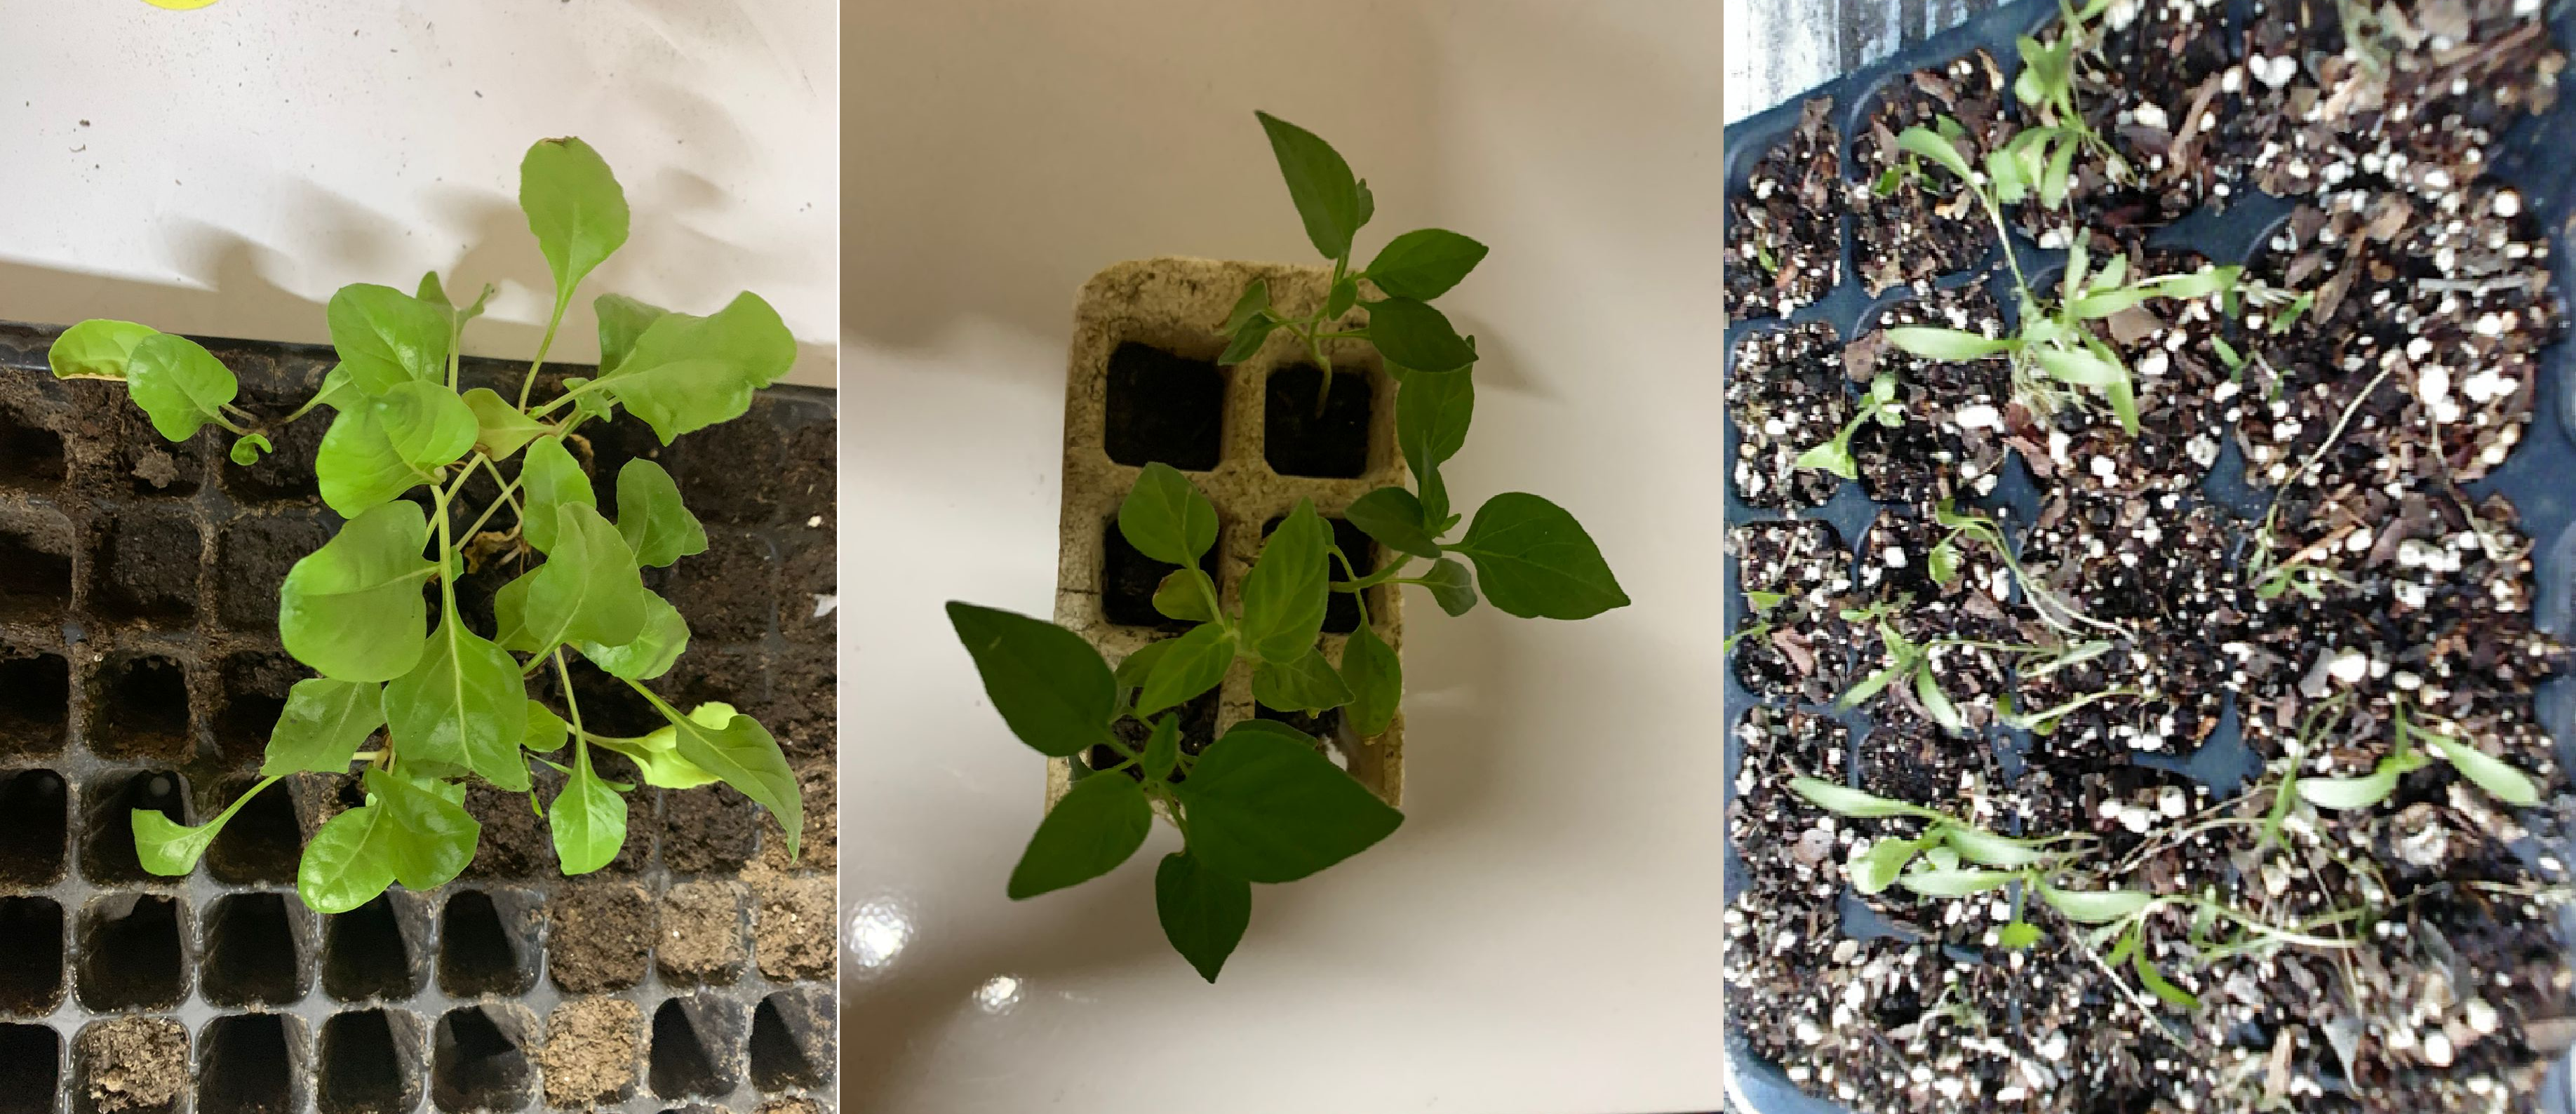
\includegraphics[scale=0.12]{imgs/plantas.png} \\
    \caption{Germinación de las plantas.}\label{plantas}
\end{figure}

\subsection{Visión por computadora}
Para el monitoreo de la germinación se programó un \textit{script} en el lenguaje de programación Python y la biblioteca OpenCV. La captura de video en tiempo real se realizó mediante una cámara web colocada sobre los semilleros con la ayuda de un tripié. La figura \ref{flujoseg} muestra el diagrama de flujo que resume las operaciones aplicadas sobre cada cuadro del video capturado para segmentar las zonas correspondientes a las plantas. Esta segmentación permitirá monitorear de manera automática el proceso de germinación de las plantas.

%\begin{itemize}
 %   \item Primeramente, se abre el ciclo de toma de video y para un mejor manejo del video se optó en convertir el espacio de color BGR a un espacio de color HSV, ya que es más fácil de trabajar en vez del espacio de color BGR. 
  %  \item Se define el rango de color que deseas segmentar, en nuestro caso pigmentos de color verde, por ende se define en función del espacio de color HSV. 
   % \item Se aplica una máscara a la toma de video original. 
    %\item Se muestra la toma original, la binarización y la segmentación del color verde.
    %\item Se realizan capturas cada día para observar el crecimiento de las plantas.
%\end{itemize}
 \begin{figure}[H]
\centering
         \includegraphics[scale=0.65]{imgs/FlujoSeg4.png} \\
    \caption{Diagrama de flujo para la segmentación de pigmentos verdes.}\label{flujoseg}
\end{figure}

%%%%%%%%%%%%%%%%%%%%%%%%%%%%%%%%%%%%%%%%%%%%%%%%%%%%%%%%%%%%%%%%%%%%%%%%%%%%%%%%%%%%%%%%%%%%%%%%%%%
%%%%%%%%%%%%%%%%%%%%%%%%%%%%%%%%%%%%%%%%%%%%%%%%%%%%%%%%%%%%%%%%%%%%%%%%%%%%%%%%%%%%%%%%%%%%%%%%%%%


\chapter{Resultados y discusión} \label{chap:AyR}
 En este capítulo, se presentarán y analizarán los resultados obtenidos a partir de los datos recopilados en la investigación. Se examinarán en detalle los hallazgos clave relacionados con la creación del controlador y el funcionamiento del sistema controlado. Además, se discutirán las implicaciones de estos resultados y se expondrán recomendaciones prácticas basadas en los objetivos planteados.

 
\section{Sistema hidropónico DFT}
Para evaluar los resultados de un sistema hidropónico DFT utilizando un controlador basado en lógica difusa se diseñó un experimento para compararlo con un sistema convencional. Se realizaron dos propuestas de sistemas: uno de 8 canales de riego y otro a 2 canales, los cuales se muestran en las figuras \ref{sistema8} y \ref{sistema8_2}. El sistema cuenta con un recipiente de 40 litros donde se encuentra la solución nutritiva donde cada hora se activa la bomba periférica y se realiza el cambio de solución en los canales de riego para oxigenarla.

 \begin{figure}[H]
\centering
         \includegraphics[scale=0.33]{imgs/1.png} \\
    \caption{Sistema hidropónico DFT propuesto de 8 canales. }\label{sistema8}
\end{figure}

 \begin{figure}[H]
\centering
         \includegraphics[scale=0.27]{imgs/dosCanales.jpg} \\
    \caption{Sistema hidropónico DFT propuesto de 2 canales. }\label{sistema8_2}
\end{figure}



\section{Pruebas funcionales del circuito de control}
El circuito de control está integrado por un microcontrolador ESP32, 4 bombas peristálticas y 4 sensores. Estos componentes están montados en una placa de acrílico. En la figura \ref{Peris}, se muestran las bombas peristálticas que fueron sujetadas por medio de soportes diseñados e impresos con filamento PLA. También se muestran los contenedores de 250 mililitros, los cuales contienen las siguientes sustancias: una solución alcalina con un pH de 10, una solución ácida con un pH de 4, un concentrado de nutrientes para el sistema y un último recipiente con agua.
 \begin{figure}[H]
\centering
         \includegraphics[scale=0.23]{imgs/perisss.jpg} \\
    \caption{Colocación de bombas peristálticas. }\label{Peris}
\end{figure}

En la figura \ref{flotador} se observan los sensores que contienen el sistema que son introducidos directamente en la solución nutritiva mediante una estructura de acrílico y flotadores que evitan que los sensores toquen el fondo del tanque y choquen con la minilavadora que se encarga del mezclado y oxigenación de la solución nutritiva.
 \begin{figure}[H]
\centering
         \includegraphics[scale=0.15]{imgs/flotador.jpg} \\
    \caption{Sensores con flotadores. }\label{flotador}
\end{figure}
La integración de todos los componentes del circuito de control en el tanque se muestran en la figura \ref{completo}. 
 \begin{figure}[H]
\centering
         \includegraphics[scale=0.15]{imgs/circuitoCompleto.jpg} \\
    \caption{Componentes del circuito de control en el tanque. }\label{completo}
\end{figure}

\section{Control de dosificación de nutrientes}
\subsection{Simulación de la curva de control}
Para la implementación del controlador, primeramente se realizó una simulación de curva de control para la comparación de los datos de salida con la salida real en el sistema.  Para ello, se utilizó el lenguaje de programación Python y mediante funciones de la biblioteca \textit{scikit-fuzzy} se definieron funciones de membresía para los valores lingüísticos de entrada establecidos en el apartado \textit{ 4.4. Control difuso para la dosificación de nutrientes}. Estos términos son utilizados de dos formas: para la conductividad eléctrica en valores de error entre [-4000,4000] y de pH con valores de error entre [-14,14]. La salida del porcentaje de PWM es la misma para las dos situaciones, con una escala de porcentaje de [-100,100]. Como método de defusificación se utiliza el método del centroide y se despliega la curva de control utilizando funciones de la biblioteca \textit{matplotlib}. Las curvas de control en el caso del pH se muestran en la figura \ref{ph2} y la curva de control para la CE en la figura \ref{conduc2}.
\begin{figure}[H]
\centering
         \includegraphics[scale=0.6]{imgs/CurvaPH_Esp.png} \\
    \caption{Curva de control para las bombas peristálticas que proveen las sustancias alcalina y ácida.}\label{ph2}
\end{figure}
\begin{figure}[H]
\centering
         \includegraphics[scale=0.6]{imgs/CurvaCE_Esp.png} \\
    \caption{Curva de control para las bombas peristálticas del suministro del concentrado de solución nutritiva y agua.}\label{conduc2}
\end{figure}

\subsection{Implementación del controlador difuso}
%%%%%%%%%%%%%%%%%%%%%%%PH-----------%%%%%%%%%%%%%%%%%%%%%%%%%%%%%%%%
Para la programación del algoritmo del control difuso en el microcontrolador ESP32 se utilizó el entorno de desarrollo Arduino. El diagrama de flujo del algoritmo programado se puede observar en la figura \ref{flujo}.

\begin{figure}[H]
\centering
         \includegraphics[scale=0.68]{imgs/Flujo (4).png} \\
    \caption{Diagrama de flujo del algoritmo de control difuso.}\label{flujo}
\end{figure}

Partiendo de la creación del algoritmo se generaron 4 casos específicos para las pruebas del controlador, que se describen a continuación. 

\subsubsection{Caso 1: Solución nutritiva con pH ácido}

En este caso, dentro del taque se realizó una disminución en el pH de la solución nutritiva llevándolo a un valor inicial cercano a 4. Como puede observarse en la gráfica superior de la figura \ref{PHMenos}, entre las muestras 18 y 32 el controlador realiza maniobras dentro del proceso en el ESP32 enviando información de porcentaje de PWM necesario para el control, como puede observarse en la gráfica central de la figura \ref{PHMenos}. Durante este proceso se puede observar que el controlador mantiene el valor de pH cerca del valor de referencia neutro de 7. Al mismo tiempo, en la gráfica inferior de la figura \ref{PHMenos} se muestra el valor de porcentaje de PWM en con una escala de voltaje entre 0 y 12 V.
\begin{figure}[H]
\centering
         \includegraphics[scale=0.85]{imgs/phMenos.png} \\
    \caption{Señales obtenidas para el caso en el que se parte de una solución nutritiva con pH alcalino. En la gráfica superior se muestran los valores de lectura obtenidos del sensor de pH; En la gráfica central se muestran los valores de salida del controlador sobre el porcentaje de PWM; En la gráfica inferior se muestran los valores de voltaje de alimentación de las bombas peristálticas.}\label{PHMenos}
\end{figure}

%%%%%%%%%%%%%%%%%%%%%%%%%%%%%%%%%%%%%%%%%%%%%%%%%%%%%%%
%%%%%%%%%%%%%%%%%%%%%%%PH++++++++++++++%%%%%%%%%%%%%%%%%%%%%%%%%%%%%%%%
\newpage
\subsubsection{Caso 2: Solución nutritiva con pH alcalino}

En este caso se partió de un valor de pH cercano a 10, como se muestra en la gráfica superior de la figura \ref{PHMas}. Al empezar a funcionar, el controlador envía el porcentaje de PWM adecuado para disminuir el pH en la solución nutritiva, como se muestra en la gráfica central de la figura \ref{PHMas}. Durante el proceso el valor de pH se mantiene en el valor de referencia neutro de 7. En la gráfica inferior de la figura \ref{PHMas} se muestran las variaciones de voltaje ocurridas durante el control del pH.
\begin{figure}[H]
\centering
         \includegraphics[scale=0.85]{imgs/phMas.png} \\
    \caption{Señales obtenidas para el caso en el que se parte de una solución nutritiva con pH alcalino. En la gráfica superior se muestran las lecturas obtenidas del sensor de pH; En la gráfica central se muestran los valores de salida del controlador sobre el porcentaje de PWM; En la gráfica inferior se muestran los valores de voltaje de alimentación de las bombas peristálticas.}\label{PHMas}
\end{figure}
%%%%%%%%%%%%%%%%%%%%%%%%%%%%%%%%%%%%%%%%%%%%%%%%%%%%%%%
%%%%%%%%%%%%%%%%%%%%%%%SolucionALTA++++++++++%%%%%%%%%%%%%%%%%%%%%%%%%%%%%%%%
\subsubsection{Caso 3: Solución nutritiva con bajo contenido de minerales}

Para el tercer caso se parte de una solución nutritiva con un nivel bajo de minerales y por lo tanto con una CE menor, con un valor inicial de alrededor de $450 \mu s/cm$, como se muestra en la gráfica superior de la figura \ref{CEMenos}. La gráfica central de la figura \ref{CEMenos} muestra el porcentaje de PWM generado por el controlador para aumentar el voltaje de alimentación de las bombas, mostrado en la gráfica inferior de la figura \ref{CEMenos}. El concentrado de minerales a usar debe ser preparado con antelación. La relación usada en esta preparación fue de 2 ml de minerales por cada litro de agua. 
\begin{figure}[H]
\centering
         \includegraphics[scale=0.75]{imgs/CEMenos.png} \\
    \caption{Señales obtenidas para el caso en el que se parte de una solución nutritiva con bajo contenido de minerales. En la gráfica superior se muestran los valores de lectura obtenidos del sensor de CE; En la gráfica central se muestran los valores de salida del controlador sobre el porcentaje de PWM; En la gráfica inferior se muestran los valores de voltaje de salida hacia las bombas peristálticas.}\label{CEMenos}
\end{figure}
%%%%%%%%%%%%%%%%%%%%%%%%%%%%%%%%%%%%%%%%%%%%%%%%%%%%%%%
%%%%%%%%%%%%%%%%%%%%%%%Solucion baja---------------%%%%%%%%%%%%%%%%%%%%%%%%%%%%%%%%
\subsubsection{Caso 4: Solución nutritiva con alta concentración de minerales}

En este último caso, a una solución nutritiva con valor de CE por debajo del límite inferior, se le agregó aproximadamente $\frac{1}{4}$ de taza de sal, ya con el sistema funcionando, para incrementar el valor de CE de alrededor de $1200 \mu s/cm$ a $4200 \mu s/cm$, como se muestra en la gráfica superior de la figura \ref{CEMas}. A diferencia del caso de donde se partió de una solución con baja concentración de sales, en este caso el controlador tardó más muestras en alcanzar el rango deseado después de haber incrementado la CE debido a que fue necesario utilizar más agua como disolvente para lograr el objetivo de control, llegando a los límites de error que pueden existir en el universo empleado. La gráfica central de la figura \ref{CEMas} muestra el porcentaje de PWM enviado por el controlador, mientras que la gráfica inferior de la figura \ref{CEMas} muestra el voltaje enviado a las bombas peristálticas correspondientes.

\begin{figure}[H]
\centering
         \includegraphics[scale=0.75]{imgs/CEMas.png} \\
    \caption{Señales obtenidas para el caso en el que se parte de una solución nutritiva con alta concentración de minerales. En la gráfica superior se muestran los valores de lectura obtenidos del sensor de CE; En la gráfica central se muestra la salida del controlador sobre el porcentaje de PWM; En la gráfica inferior se muestra el voltaje de salida hacia las bombas peristálticas.}\label{CEMas}
\end{figure}

%%%%%%%%%%%%%%%%%%%%%%%%%%%%%%%%%%%%%%%%%%%%%%%%%%%%%%%
\section{Monitoreo de variables}

Para poder monitorear las variables a distancia mediante el protocolo MQTT, fue necesario configurar un \textit{broker} (figura \ref{broker}). 
Por medio del \textit{broker}, se enlazan las interfaces mediante una suscripción a un tópico, y el \textit{broker} se encarga de distribuir la información recibida entre todos los componentes que están suscritos a dicho tópico. El microcontrolador ESP32 se encarga de obtener las lecturas de los sensores, y publicarlas en la plataforma Node-Red para su posterior distribución. La aplicación móvil recibe las notificaciones de las lecturas publicadas, ya que es un dispositivo que también está suscrito a dichos tópicos. En las figuras \ref{servidor} y \ref{app}, se muestra el estado de las interfaces cuando ya están suscritas a dichos tópicos y cuando el sistema ya está en operación. Las interfaces despliegan gráficas que dan evidencia del comportamiento de los sensores en función del tiempo.   
%Para ello se enlazan cada una de las interfaces al suscribirse al \textit{broker} y este mismo distribuye la información publicada por el ESP32 hacia el servidor Node-Red y la aplicación móvil, como se observa en las figuras \ref{servidor} y \ref{app} respectivamente. La información de los parámetros se obtienen de los sensores que se encuentran en la solución nutritiva, dichos parámetros son: la temperatura, la humedad, la conductividad eléctrica y el pH de la solución.

 \begin{figure}[H]
\centering
         \includegraphics[scale=0.7]{imgs/broker.jpeg} \\
    \caption{Publicación de datos en el \textit{broker} mosquitto.}\label{broker}
\end{figure}
\begin{figure}[H]
\centering
         \includegraphics[scale=0.4]{imgs/servidor1.jpeg} \\
    \caption{Visualización de las lecturas obtenidas mediante la interfaz web proporcionada por la plataforma Node-red.} \label{servidor}
\end{figure}

\begin{figure}[H]
\centering
         \includegraphics[scale=0.5]{imgs/app1.jpeg} \\
    \caption{Visualización de las lecturas obtenidas mediante la aplicación móvil vinculada con la plataforma Node-Red.} \label{app}
\end{figure}



\section{Monitoreo de germinación}

\subsection{Visión por computadora}
Para el monitoreo de germinación de las plantas se programó un \textit{script} en el lenguaje de programación Python con las bibliotecas de OpenCV, el cual realiza la captura de video en tiempo real utilizando una cámara web, que se encuentra dirigida hacia los semilleros. En este \textit{script} se implementa un método de segmentación, donde sobre cada cuadro del video se realiza un cambio del espacio de colores BGR a HSV. Enseguida se genera una máscara binaria correspondiente a los tonos en verde observado en el semillero con la cual se segmentan las zonas correspondientes a las plantas. Al realizar capturas cada día y compararlas se puede observar el crecimiento de las plantas. Los resultados de este proceso se puede observar en las figuras \ref{cam}, \ref{foto} y \ref{segmentacion}.

\begin{figure}[H]
\centering
         \includegraphics[scale=0.2]{imgs/Camara.jpg}
    \caption{Colocación de la cámara en los semilleros.}\label{cam}
\end{figure}

\begin{figure}[H]
\centering
         \includegraphics[scale=0.2]{imgs/fotoCamara.jpg}
    \caption{Fotografía de los semilleros.}\label{foto}
\end{figure}

\begin{figure}[H]
\centering
         \includegraphics[scale=0.35]{imgs/germinacion.jpeg}
    \caption{Segmentación de las plantas germinadas.}\label{segmentacion}
\end{figure}

\section{Discusión}
La implementación de algoritmos de control difuso en los sistemas hidropónicos es una estrategia que permite controlar los nutrientes de importancia en el crecimiento de las plantas, buscando mejorar la producción.

Sin embargo, es importante señalar algunos desafíos asociados con la implementación del control difuso en sistemas hidropónicos. Por un lado, se debe tener conocimientos técnicos acerca del tema para la configuración inicial de los conjuntos de reglas difusas y los parámetros del controlador. Además, la precisión del control difuso puede depender en gran medida de la calidad y la confiabilidad de los sensores y actuadores utilizados.

Por otro lado, la utilización de un control difuso presenta un enfoque prometedor para maximizar la productividad de los cultivos. Si se implementa y ajusta correctamente, esta técnica puede contribuir significativamente al control automático de sistemas hidropónicos usados en agricultura. Sin embargo, se deben realizar más experimentos con otros tipos de sistemas de agricultura en interiores para comprobar su eficacia en estos casos.

\section{Análisis de costos del proyecto}
El análisis de costos del proyecto se llevó a cabo tomando los aspectos más importantes dentro del sistema, incluyendo los materiales de la estructura hidropónica y del circuito de control. Este análisis se basa en los precios obtenidos el día 5 de mayo del 2023 en pesos mexicanos. El tiempo de construcción del sistema, ya teniendo todos los componentes y herramientas fue de alrededor de 5 días.

\textbf{Sistema hidropónico DFT de 8 canales}

\begin{table}[H]
\centering
\caption{Análisis de costos del sistema a 8 canales.} 
\begin{tabular}{|p{4.7cm}|p{1.85cm}|p{2.5cm}|p{1.8cm}|p{2.2cm}|}
\hline
           \textbf{Material} & \textbf{Cantidad} & \textbf{Unidad} & \textbf{Costo unitario} & \textbf{Costo total} \\
\noalign{\hrule height 2pt}

        Tubo PVC de 3 pulgadas &  22  & Metros & \$29.00& \$638.00  \\
        \hline
        Codo PVC de 3 pulgadas &  8 & Pieza & \$15.00& \$120.00\\
       \hline
        T PVC de 3 pulgadas &  23 & Pieza & \$25.00& \$575.00\\
     \hline
      Tubo hidráulico de 1 pulgadas &   4.5 & Metros & \$30.00& \$135.00  \\
        \hline
        Codo de 1 pulgadas &  4 & Pieza & \$10.00& \$40.00\\
       \hline
        T de 1 pulgadas &  8 & Pieza & \$10.00& \$80.00\\
         \hline
     Cople Tipo Hembra 1 pulgada & 1   & Pieza & \$10.00& \$10.00 \\
          \hline
     Cople Tipo Macho 1 pulgada & 3  & Pieza & \$10.00& \$30.00\\
           \hline
     Llave de paso 1 pulgada & 9  & Pieza & \$65.00& \$585.00 \\
            \hline
     Tubo cristalino 1 pulgada & 3  & Metros & \$40.00& \$120.00 \\
            \hline
     Pegamento para PVC & 2  & Pieza & \$190.00& \$280.00 \\
            \hline
     Canastilla de 2 pulgadas & 44  & Pieza & \$9.00& \$396.00 \\
            \hline
      &   &  &  \textbf{Total :}& \$3009.00 \\
            \hline

       

\end{tabular}
\label{tab:t3}
\end{table}

\newpage
\textbf{Sistema hidropónico DFT de 2 canales.}

\begin{table}[H]
\centering
\caption{Análisis de costos del sistema a 2 canales.} 
\begin{tabular}{|p{4.7cm}|p{1.85cm}|p{2.5cm}|p{1.8cm}|p{2.2cm}|}
\hline
      \textbf{Material} & \textbf{Cantidad} & \textbf{Unidad} & \textbf{Costo unitario} & \textbf{Costo total} \\
\noalign{\hrule height 2pt}

        Tubo PVC de 3 pulgadas &  14  & Metros & \$29.00& \$406.00  \\
        \hline
        Codo PVC de 3 pulgadas &  8 & Pieza & \$15.00& \$120.00\\
       \hline
        T PVC de 3 pulgadas &  10 & Pieza & \$25.00& \$250.00\\
     \hline
      Tubo hidráulico de 1 pulgadas &   2.5 & Metros & \$30.00& \$75.00  \\
        \hline
        Codo de 1 pulgadas &  4 & Pieza & \$10.00& \$40.00\\
       \hline
        T de 1 pulgadas &  2 & Pieza & \$10.00& \$20.00\\
         \hline
     Cople Tipo Hembra 1 pulgada & 1   & Pieza & \$10.00& \$10.00 \\
          \hline
     Cople Tipo Macho 1 pulgada & 3  & Pieza & \$10.00& \$30.00\\
           \hline
     Llave de paso 1 pulgada & 3  & Pieza & \$65.00& \$185.00 \\
            \hline
     Tubo cristalino 1 pulgada & 1  & Metros & \$40.00& \$40.00 \\
            \hline
     Pegamento para PVC & 1  & Pieza & \$155.00& \$155.00 \\
            \hline
     Canastilla de 2 pulgadas & 11  & Pieza & \$9.00& \$99.00 \\
            \hline
      &   &  &  \textbf{Total :}& \$1430.00 \\
            \hline


\end{tabular}
\label{tab:t4_r}
\end{table}
\newpage
\textbf{Circuito de control}

\begin{table}[H]
\centering
\caption{Análisis de costos del circuito de control.} 
\begin{tabular}{|p{4.7cm}|p{1.85cm}|p{2.5cm}|p{1.8cm}|p{2.2cm}|}
\hline
                  \textbf{Material} & \textbf{Cantidad} & \textbf{Unidad} & \textbf{Costo unitario} & \textbf{Costo total} \\
\noalign{\hrule height 2pt}

        Microcontrolador ESP32 & 1   & Pieza & \$209.00& \$209.00  \\
        \hline
        Raspberry pi 3 b+ &  1 & Pieza & \$2045.00& \$2045.00\\
       \hline
     Sensor Dht11 &  1 & Pieza & \$65.00& \$65.00\\
     \hline
     Sensor PH-4502C & 1 & Pieza & \$535.00& \$535.00\\
     \hline
     Sensor TDS meter v1 &  1& Pieza & \$630.00& \$630.00\\
      \hline
     Sensor DS18B20 &   1 & Pieza & \$58.00& \$58.00\\
         \hline
     Driver Puente H L298N & 2   & Pieza & \$75.00& \$150.00 \\
          \hline
     Modulo relé de 2 canales & 1  & Pieza & \$150.00& \$150.00\\
           \hline
     Bombas peristálticas  & 4  & Pieza & \$122.00& \$488.00 \\
            \hline
             Bomba periférica 1/2 Hp & 1  & Pieza & \$436.00& \$436.00 \\
            \hline
             Minilavadora & 4  & Pieza & \$205.00& \$205.00 \\
            \hline
      &   &  &  \textbf{Total :}& \$4971.00 \\
            \hline

       

\end{tabular}
\label{tab:t5}
\end{table}


%%%%%%%%%%%%%%%%%%%%%%%%%%%%%%%%%%%%%%%%%%%%%%%%%%%%%%%%
%%%%%%%%%%%%%%%%%%%%%%%%%%%%%%%%%%%%%%%%%%%%%%%%%%%%%%%%%%%%%%%%%%%%%%%%%%%%%%%%%%%%%%%%%%%%%%%%%%%



\chapter{Conclusiones y trabajo futuro} 
\label{chap:CyTF}


La agricultura es una de las actividades que tienen un gran impacto en la economía del país. La hidroponía es una técnica agrícola altamente eficiente y prometedora que ofrece numerosos beneficios en comparación con los métodos tradicionales. Es importante destacar que la implementación exitosa de la hidroponía requiere un conocimiento acerca de los principios agrícolas, así como una supervisión y ajuste continuos de los factores ambientales. Además, no todos los cultivos son igualmente adecuados para este sistema y es esencial considerar las características específicas de cada planta y del entorno en el cual se desee cultivar.

A lo largo de la investigación, se ha explorado cómo la hidroponía elimina las restricciones de las limitaciones de suelo y clima, permitiendo un control preciso sobre factores como la nutrición, el pH, la humedad y la temperatura, a través del diseño y puesta en operación de un controlador basado en lógica difusa, el cual fue el objetivo fundamental de este trabajo de investigación. La implementación de las tecnologías ha logrado un punto en el cual la automatización de estos sistemas y la aplicación de técnicas de IoT, ayudan a conocer datos importantes de las plantas en el sistema hidropónico en tiempo real. Se logró desarrollar un controlador difuso para automatizar el control de un prototipo de sistema hidropónico y también la aplicación de técnica de IoT para realizar el monitoreo contante de plantas sembradas/montadas en un sistema hidropónico.
   
Aunque la inversión inicial puede ser más alta debido a la infraestructura necesaria, los costos a largo plazo se reducen mediante un uso eficiente de recursos y una producción constante. La tecnología moderna ha permitido automatizar muchos aspectos de los sistemas hidropónicos, lo que hace que la gestión sea más accesible incluso para personas que no están familiarizadas con conceptos y técnicas de agricultura hidropónica.
En última instancia, la elección de un sistema hidropónico como el DFT dependerá de los objetivos a alcanzar, el tipo de cultivo que se desea cultivar y las condiciones climáticas específicas en las que se instalará. Como con cualquier tipo de sistema alternativo de agricultura, es importante considerar cuidadosamente las ventajas y desventajas en relación con las necesidades y recursos disponibles.
\newpage

Respecto al trabajo futuro se definieron las siguientes actividades: 
%\textcolor{green}{\textbf{(DAVID: Con respecto a estos puntos, deberia haber una propuesta y lo que se espera encontrar. Por ejemplo: ``Incrementar mi actividad fisica, lograr\'ia tener un impacto en mi IMC, lo cual pudiera reducir en el dolor de mis rodillas. - le encargo pensar este punto '' }}
%\begin{itemize}
 %   \item Probar o explorar distintas fórmulas nutricionales para determinar cual proporciona mejor rendimiento para cierto grupo de cultivos en particular.
  %  \item Realizar comparativas de crecimiento y rendimiento.
   % \item Generar un control de germinación utilizando visión por computadora.
    %\item Comparación de su uso con otros tipos de sistemas.
%\end{itemize}
\begin{itemize}
    \item Probar o explorar distintas fórmulas nutricionales para identificar la que mejora el rendimiento para un grupo de cultivos en particular.
    \item Realizar comparativas de crecimiento y rendimiento utilizando los distintos tipos de métodos de germinación para obtener información relevante para esta etapa y mejorar la producción de sembradíos.
    \item Complementar el programa de visión por computadora con algoritmos de inteligencia artificial para monitorear automáticamente la etapa de germinación y ciclo de cosecha buscando detectar enfermedades y dar seguimiento al crecimiento de las plantas.
    \item Probar el controlador difuso propuesto en otros sistemas de agricultura en interiores y en otras configuraciones de sistemas hidropónicos.
\end{itemize}






\bibliographystyle{acm}
\bibliography{bibiliography/referencia-tesis}
% En vez de los dos comandos anteriores
%\printbibliography


\end{document}
